\documentclass[10pt,authoryear]{elsarticle}
\usepackage{calc,amsmath,amssymb,amsfonts}
\usepackage[LGR,T1]{fontenc}
\usepackage{lmodern}
\usepackage[spanish,es-tabla]{babel} 
\usepackage{xcolor,fancyhdr}
%\usepackage[top=1in,bottom=0.5in,hmargin=1in,nohead,includefoot,foot=0.5in,footskip=0.9602in]{geometry}
\usepackage[output-decimal-marker={.}]{siunitx}
\decimalpoint
\usepackage{enumitem,hyperref}
\hypersetup{colorlinks=true,allcolors=blue,pdfauthor=IVM}
% Outline numbering
\setcounter{secnumdepth}{1}
% Pages
\fancypagestyle{Convertedi}{\fancyhf{}
	\fancyhead[L]{}
	\fancyfoot[L]{\thepage{}}
	\renewcommand\headrulewidth{0pt}
	\renewcommand\footrulewidth{0pt}
	\renewcommand\thepage{\arabic{page}}
}
\fancypagestyle{Standard}{\fancyhf{}
	\fancyhead[L]{}
	\fancyfoot[L]{}
	\renewcommand\headrulewidth{0pt}
	\renewcommand\footrulewidth{0pt}
	\renewcommand\thepage{\arabic{page}}
}
\fancypagestyle{Convertedii}{\fancyhf{}
	\fancyhead[L]{}
	\fancyfoot[C]{\thepage}
	\renewcommand\headrulewidth{0pt}
	\renewcommand\footrulewidth{0pt}
	\renewcommand\thepage{\arabic{page}}
}

\author{ }
\date{ }
\usepackage[margin=1in]{geometry} % Sets wide 1-inch margins
\usepackage{setspace}              % Required for line spacing
\usepackage{lineno}                % Required for line numbers

%\doublespacing                     % Applies double-spacing throughout
%\linenumbers 
\usepackage{multirow}
\usepackage{array}
%Dirección de la imágenes
\graphicspath{ {Images/} }
\usepackage{subcaption}
\usepackage{amsmath, amssymb, bm, mathtools, mathdots}
\newcommand{\R}{\mathbb{R}} %\R for reelle tal
\newcommand{\C}{\mathbb{C}} %\C for komplekse tal
\newcommand{\N}{\mathbb{N}} %\N for naturlige tal
\newcommand{\Z}{\mathbb{Z}} %\Z for hele tal
\newcommand{\Q}{\mathbb{Q}} %\Q for rationale tal


\usepackage{tikz}
\usetikzlibrary{automata, positioning, arrows.meta, calc}

\tikzset{every picture/.style={line width=0.75pt}}

\usepackage{nicematrix}
\usepackage{pgfgantt}





\begin{document}
	\clearpage
	\pagestyle{Convertedii}
	\iffalse
	{\centering\color{black}
		\textbf{Highlights}\textbf{\textsuperscript{*}}
		\par}
	
	
	\bigskip
	
	\begin{enumerate}[series=listWWNumvi,label=\arabic*.,ref=\arabic*]
		\item {\color{black}
			Include 3 to 5 bullet points that convey the main findings of the work.}
		\item {\color{black}
			Methods and results are not “findings,” so they should not appear as highlights.}
		\item {\color{black}
			Bullets are limited to a maximum of 85 characters, including spaces.}
		\item {\color{black}
			Bullets should be complete sentences, not sentence fragments.}
		\item {\color{black}
			Highlights should be able to stand alone, so avoid acronyms or specialized terms.}
	\end{enumerate}
	
	\bigskip
	
	
	\bigskip
	
	{\color{black}
		* Please note: Highlights are not part of the manuscript document but should be submitted in a separate editable file in
		the online submission system.  Please use “Highlights” in the file name.}
	
	{\color{black}
		Also, in the submission$\text{\textgreek{’}}$s cover letter, authors should clearly state what are the key contributions
		of their work and why their contributions are novel and worthy of journal consideration.}
	\fi
	
	\bigskip
	
	\clearpage
	\pagestyle{Convertedii}
	\setcounter{page}{1}
	{\centering\color{black}
		\textbf{Modelación probabilística de periodos de siembra del maíz en condiciones de cambio climático. Caso de estudio en Alemania.}
		\par}
	
	{\centering\bfseries\color{black}
		Isaac Vázquez-Mendoza\textsuperscript{a}*, Magali Arellano-Vazquez\textsuperscript{a}
		\par}
	
	{\color{black}
		\textsuperscript{a} 
		INFOTEC, Centro de Investigación e Innovación en Tecnologías de la Información y Comunicación, Aguascalientes 20326, Mexico.}
	
	
	\iffalse
	{\color{black}
		\textbf{*} 
		Corresponding author.}
	\fi
	{\color{black}
		\iffalse
		\textit{E-mail addresses}: \url{isaacvazquezmendoza@gmail.com} (I. Vázquez-Mendoza), \url{magali.arellano@infotec.mx} (M. Arellano-Vazquez).
	
		
		\bigskip
		
		{\color{black}
			\textbf{Abstract}}
		
		{\color{black}
			
			Understanding the evolution of agricultural systems under climatic variability is crucial for ecological management. Sowing decisions directly impact seedling emergency, crop establishment and, yield stability. These decisions rely on environmental conditions and climatic patterns, requiring integrative modeling approaches.
			To emulate agricultural practices shaped over time, a graph-based representation is proposed, in which a stochastic process evolves over the graph to determine sowing dates. The model is developed for the region-specific agro ecological conditions of Saxony, Brandenburg, and Bavaria, three German states with differentiated crop calendars.
			Days of the year are represented as nodes in a cyclic graph, together with an additional absorbing node accounting for crop establishment failure before emergence. Weights on directed edges encode environmental conditions and crop establishment dynamics, while transitions are determined by a Bernoulli-type decision at each step. The proportion of trajectories that avoid absorption quantifies the sowing suitability of each day.
			The proposed framework is scoped to the period from sowing through crop emergence. By simulating random walk realizations for every day of the year, empirical probabilities are elicited, defining sowing windows and emulating the trial-and-error development of historical crop management strategies.
			Results revealed distinct sowing windows for Saxony, Brandenburg, and Bavaria, reflecting the agro ecological specificity of each region. The estimated sowing windows also exhibited a progressive shift toward earlier calendar dates and a reduction in their duration over time, indicating increasingly narrow opportunities for successful crop establishment under climatic variability.
			These findings establish an ecologically grounded probabilistic framework for identifying sowing windows under climatic variability, focusing exclusively on the crop establishment phase from sowing to emergence.
			
			\iffalse
			A concise and factual Abstract is required, which should not be longer than 400 words. \ An Abstract should succinctly summarize a paper$\text{\textgreek{’}}$s content, including: the purpose of the research, the methods employed,
			principal results, and major conclusions/findings. \ Results should be described in specific terms, using numbers where appropriate and avoiding statements such as, “Results of our tests were good” or “Implications are discussed.” \ Because an Abstract provides a summary of the paper, there is no need to include a summary section or paragraph near the end of the paper, e.g., in the Conclusions section. \ An Abstract is often presented separately from the article,
			so it must be able to stand alone. \ For this reason, literature references should be avoided, but if essential, then cite the author(s) and year(s). \ Also, nonstandard or uncommon abbreviations or acronyms should be avoided, but if
			essential they must be defined at their first mention in the Abstract itself.
			\fi
		}
		
		
		\bigskip
		
		{\color{black}
			\textbf{\textit{Keywords.}} Sowing time; Maize; Agro climatic database; Phenology; Modeling.}
		
		\fi 
		\bigskip
		
		\section{Introducción}
		
		Las flores, frutas, vegetales y hongos representan un pilar fundamental en la cadena alimentaria \citep{Cassani_2022}. La industria agrícola, responsable de su producción continua, enfrenta desafíos crecientes debido a la incertidumbre respecto a las condiciones de cultivo, las cuales se han visto afectadas, en gran parte, por el cambio climático \citep{Parajuli_2019}.\\

Las alteraciones que se derivan del cambio climático repercuten en diversos aspectos, entre ellos, el ciclo de producción agrícola, debido a variaciones inusuales e inesperadas en temperatura, precipitación y patrones de migración de polinizadores, entre otros factores. Los cuales, en conjunto, han modificado las zonas, temporadas y rendimiento de los cultivos \citep{Bayable_2021, Cuevas_2021, Parajuli_2019}.\\

La estabilidad de los procesos productivos depende de cierta consistencia en las condiciones ambientales. Sin embargo, las variaciones a las que nos enfrentamos actualmente, derivadas principalmente por el cambio climático, repercuten en dicha consistencia, incrementando la inestabilidad en la seguridad alimentaria y el desabasto a la par de reducir la producción y exportación, impactando directamente la economía de las naciones \citep{Farooq_2022}.\\

Cada cultivo prospera dentro de umbrales agroambientales específicos, que en muchos casos, han sido ya ampliamente descritos con anterioridad en la literatura científica; e.g., el aguacate \citep{Moraes_2022, Rocha-Arroyo_2011} o el agave \citep{García-Mendoza_2002}. El maíz (\textit{Zea mays}), un cultivo de origen mexicano \citep{OrozcoRamrez_2016}, representa un caso particular al ser considerado como uno de los cultivos más importantes a nivel mundial para el abastecimiento alimenticio directo e indirecto y sus usos industriales \citep{Revilla_2022}.\\

El maíz ha sido empleado para consumo tanto de dieta primaria como de dieta secundaria; i.e., incorporado en conjunto con otros alimentos o para forrajeo \citep{Revilla_2022}. Asimismo, este cultivo se emplea en diversas actividades del sector productivo y de manufactura \citep{Ranum_2014}; e.g., cervezas, jarabes, harinas, medicamentos y biocombustibles \citep{Rausch_2006,SOKANADEAGA_2024, Zhang_2022}.\\


A nivel mundial, el consumo de las distintas variedades de este cultivo aporta, en promedio, el $5.3\%$, el $4.6\%$ y $1.6\%$ de la ingesta calórica, proteica y grasa, respectivamente, per capita diaria \citep{Erenstein_2022}. Las variedades del maíz pueden clasificarse por su tamaño, dulzor, composición del endospermo, color o tasa de maduración \citep{Ranum_2014}; no obstante, comparten su respuesta a las condiciones de cultivo \citep{Baum_2019, Sanchez_2014, Parent_2012}.\\


Los calendarios agrícolas proporcionan información crítica sobre cuándo se llevan a cabo las etapas de desarrollo del cultivo que conforman su fenología \citep{Franch_2022}. De esta manera, se organiza el manejo agrícola tanto de la secuencia fenológica completa como de etapas particulares; e.g., la siembra o la cosecha.\\

A través del alza en la frecuencia de eventos climáticos extremos \citep{MIRON_2023}, el incremento de la temperatura promedio del planeta \citep{Shivanna_2022} y los desfases en la duración de las estaciones del año \citep{Wang_2014}, el cambio climático ha alterado la distribución espacial de las zonas de cultivo \citep{SU_2023} y los calendarios agrícolas \citep{Franch_2022}.\\


Lo anterior impone a la agricultura un reto para garantizar la calidad y la cantidad de productos para satisfacer las necesidades alimentarias en el futuro \citep{MIRON_2023}. Por otro lado, se ha observado que, para el maíz, las fechas de siembra juegan un rol determinante en la cosecha resultante \citep{Baum_2019, BernalMorales_2025, Long_2017, Mason_2018, Parker_2016, Sacks_2011}.\\


De acuerdo con \cite{Sanchez_2013}, el periodo de la siembra a la emergencia de la plántula es una de las temporadas más susceptibles de este cultivo. Por tanto, este trabajo se centra en proponer una recalendarización del periodo de siembra que garantice una baja exposición al estrés ambiental durante el ciclo de desarrollo comprendido hasta la emergencia.\\

Anualmente se destinan aproximadamente 200 millones de hectáreas (M ha) para la plantación de maíz, de las cuales, aproximadamente el 9\% se ubica en Europa \citep{Erenstein_2022}. No obstante, a consecuencia del cambio climático, las regiones con mayor altitud y aquellas al norte de la región noroeste de Europa, en particular Alemania, tendrán un incremento en las zonas con potencial de producción agrícola del maíz \citep{Miedaner_2021}.\\

Esta transición implica retos en tanto a la renovación de la planeación, la gestión, el desarrollo y la correcta implementación de las técnicas agrícolas relativas al manejo y cuidado del cultivo \citep{Parent_2018, DONMEZ_2023}. La identificación de periodos de siembra, bajo la transición que supone el cambio climático, continúa siendo limitada, no por desinterés sino por la tendencia a considerarlas estáticas \citep{Parker_2016}, la complejidad inherente a la incertidumbre climática \citep{Waha_2011} y por falta de especificidad en la información disponible correspondiente a las fechas de plantación  \citep{Portmann_2010, Sacks_2010}.\\

 En este sentido, este estudio pretende robustecer la planificación de las fechas de siembra del maíz mediante la implementación de herramientas analíticas y computacionales para la toma de esta decisión, ante la necesidad de adaptar la planificación agrícola a los cambios esperados en las condiciones ambientales futuras. El estudio se focaliza en el sureste de Alemania, una región que alberga aproximadamente el 54.42\% de las 9.5 M ha de superficie empleada anualmente para la producción de los principales cultivos \citep{Duden_2024}.\\

La expansión proyectada de su área potencial de cultivo en regiones como Alemania, la estabilidad nutricional bajo escenarios de elevadas concentraciones atmosféricas de CO$_2$ \citep{Myers_2014} y su papel en la seguridad alimentaria global \citep{TANUMIHARDJO_2020}, en conjunto, consolidan al maíz como un cultivo estratégico no solo por su relevancia productiva y económica ante el cambio climático.\\


En consecuencia, este trabajo busca cubrir la necesidad de actualizar la planificación agronómica del periodo comprendido de la siembra a la emergencia. Determinando, mediante el análisis de datos agroclimáticos históricos, aquellas temporadas favorables para el desarrollo, mitigando el efecto del cambio climático.

		
		\iffalse
		{\color{black}
			An Introduction should contain three components: (1) one or more paragraphs describing the problem, which justifies, and provides a context for, the research, (2) a concise review of pertinent past international research related to the problem and how the current study expects to extend those prior results, and (3) objectives for the current research program and/or current study reported (possibly along with a “roadmap” of the paper that previews its contents for the reader). \ The literature review portion (\#2 above) should include author synthesis and evaluation of past research, rather than solely enumerating a list of past studies. \ The authors should clearly describe gaps in the current state of the science, and how the current paper will contribute something new to the scientific body of knowledge (i.e., mitigate or eliminate knowledge gaps). \ Detailed methods, or results, of the current study should not appear here. \ With such a logical structure and appropriate segue sentences, subheadings are unnecessary. \ There is also no need for a separate Related Work or Literature Review or Background section. }
		
		{\color{black}
			Manuscripts should be prepared with consecutive line numbering (required), with wide margins and double-spacing throughout (required), i.e., also for abstracts, footnotes, and references. \ Every page of the manuscript, including the title page, references, tables, etc. should be numbered. \ However, in the text, no reference should be made to page numbers; if necessary, one may refer to sections. \ Avoid excessive use of italics to emphasize parts of the text.}
		
		{\color{black}
			Divide your article into clearly defined and numbered sections. \ Subsections should be numbered 1.1 (then 1.1.1, 1.1.2, ...), 1.2, etc. (the Abstract is not included in section numbering). \ Also, use this numbering for internal cross-referencing; do not just refer to “the text.” \ Every subsection should be given a brief heading. \ Each heading should appear on its own separate line.}
		
		{\color{black}
			The use of acronyms is merely a shorthand convenience. \ Their use does not relieve authors from the responsibility of matching noun-verb case, and adjective-noun case. \ If “UAV” is defined as singular, for example “unmanned aerial vehicle,” then all uses of that acronym should be singular, and the plural form would be {\textquotedbl}UAVs.” \ If one defines an acronym in the plural case, the recommended way to do so is by adding an “s” at the end, as in, “…unmanned aerial vehicles (UAVs)…” to facilitate using the acronym both as singular (UAV) and plural (UAVs).  While acronyms appear in capital letters, the terms they represent should not generally be capitalized unless they are proper nouns, e.g., “unmanned aerial vehicle,” “deep learning,” and “convolutional neural network” are not proper nouns. \ Acronyms that are used (and necessary) in the Abstract and in the manuscript proper need to be defined in both places. \ Also, acronyms should NOT be used in the title, keywords, or highlights, unless they are readily understood by the readership. \ Finally, acronyms should ONLY be defined for \textit{terms used frequently} in a manuscript; do not define an acronym for a term that is only used a few times (especially in the Abstract). \ A manuscript containing many acronyms is difficult for the readership, as they must actively translate unfamiliar acronyms back to the terms they represent.}
		\fi
		
		\bigskip
		
		
		\section{Materiales y métodos}
		
		\subsection{Bases de datos}
\label{subsection:Database}

Para integrar las condiciones ambientales que caracterizan el periodo comprendido entre la siembra y la emergencia del maíz, en este trabajo se emplean las bases de datos ráster desarrolladas por el Servicio Meteorológico Alemán (DWD, por sus siglas en alemán). Estas bases de datos son generadas mediante técnicas y modelos de interpolación previamente establecidos y se encuentran sujetas a procesos continuos de mantenimiento y control de calidad por parte del DWD.\\

Al contar con cobertura nacional de Alemania, alta resolución espacial, consistencia metodológica, amplia disponibilidad de datos históricos y soporte institucional, estas bases de datos constituyen fuentes de información confiables para la incorporación de registros agroclimáticos y favorecen la reproducibilidad de los resultados.\\

\subsubsection{HYRAS}

El repositorio Hydrometeorologische Rasterdatensätze (HYRAS), versión v6-1, alberga las bases de datos históricos referentes a la temperatura ambiente \citep{DWD_HYRAS_MaxTemp, DWD_HYRAS_MeanTemp, DWD_HYRAS_MinTemp} y la humedad relativa \cite{DWD_HYRAS_RelHumidity} a nivel nacional. Empleando los registros diarios, desde 1951 a la fecha, medidos a través de 1300 estaciones climáticas distribuidas en Alemania y sus siete países vecinos \citep{Razafimaharo_2020}, se genera un archivo ráster por día, con una resolución espacial de $1\times1$ km, a partir de la metodología de interpolación propuesta por \cite{Krhenmann_2016}\\



Las bases de datos en HYRAS han sido sometidas a una extensa validación. A distintas escalas temporales (día, mes, año y el periodo completo de observación), se han comparado las mediciones registradas en las estaciones con los valores interpolados correspondientes a la celda más cercana así como a lo largo de los distintos niveles de elevación del terreno \citep{Razafimaharo_2020}. Asimismo, de acuerdo con \cite{Razafimaharo_2020}, las bases de datos de este repositorio han sido comparadas con bases de datos homólogas, como el Gridded European Climate Assessment y el conjunto de datos mensuales del DWD.\\

Estas evaluaciones han demostrado una alta fidelidad entre las bases de datos del repositorio HYRAS y las correspondientes observaciones \textit{in situ}. Sin embargo, la precisión de la interpolación puede disminuir en regiones con topografía compleja, particularmente para la humedad relativa, mientras que para la temperatura conserva datos altamente comparables \citep{Razafimaharo_2020}.\\

Del repositorio HYRAS, se emplean las bases de datos de temperatura media \citep{DWD_HYRAS_MeanTemp} y humedad relativa \citep{DWD_HYRAS_RelHumidity} a lo largo de este trabajo al ser variables ambientales que participan durante el periodo fenológico comprendido entre la siembra y la emergencia del maíz.\\

Además, las características como el formato ráster, la rigurosidad metodológica, el control de calidad en los datos y la resolución espacial, permiten una representación homogénea de las condiciones ambientales en el espacio y el tiempo que resulta adecuada para análisis agrícolas a escala regional al reducir las inconsistencias asociadas con los registros de estaciones individuales.\\

\subsubsection{Ráster diarios de la temperatura del suelo a una profundidad de 5 cm}

El modelo AMBETI es una herramienta multipropósito diseñada para simular las interacciones suelo-planta-atmósfera, incluyendo el transporte de vapor de agua y agua líquida a través del suelo, así como los flujos netos de radiación en las superficies de la planta y del suelo \citep{Braden_1995}. Específicamente, la componente de termodinámica del suelo es utilizado por el DWD para estimar la temperatura diaria del suelo a una profundidad de 5 cm desde 1991, dando lugar a este conjunto de datos.\\


A partir de la interpolación de mediciones \textit{in situ} provenientes de aproximadamente 280 estaciones distribuidas en Alemania, se generan archivos ráster ASCII diarios con resolución de $1\times1$ km. La temperatura del suelo se estima inicialmente en las estaciones meteorológicas mediante el modelo AMBETI y posteriormente se interpola mediante una regresión lineal múltiple regional basada en la longitud, latitud y elevación, seguida de una triangulación para generar datos espaciales continuos sobre Alemania \citep{DWD_soiltemperature}.\\

De acuerdo con \cite{DWD_soiltemperature}, las interpolaciones resultantes son físicamente factibles dado que la temperatura del suelo está determinada principalmente por la temperatura atmosférica y la radiación solar incidente, como señalan \cite{BAUMBERGER_2024}. En consecuencia, la temperatura del suelo tiende a presentar una baja variabilidad \citep{DWD_soiltemperature}.\\ 


Lo anterior sustenta la validez metodológica de la interpolación en conjuntos de datos en formato de ráster \citep{Schloeder_2001}. Por lo tanto, el procedimiento de interpolación proporciona estimaciones espaciales confiables en Alemania, siendo la principal fuente de incertidumbre durante el invierno la distribución espacial heterogénea de la cobertura de nieve \citep{DWD_soiltemperature}.\\

Para el desarrollo de este trabajo, se seleccionó esta base de datos debido a que representa de manera cercana el ambiente térmico experimentado por las semillas de maíz durante el periodo comprendido entre la siembra y la emergencia. Asimismo, su disponibilidad diaria, cobertura nacional, resolución espacial y metodología de estimación basada en principios físicos robustece la representación de las condiciones ambientales que influyen en el periodo de siembra a emergencia de la secuencia fenológica.\\

\subsubsection{Ráster diarios de la humedad del suelo para el maíz en Alemania}

La base de datos de humedad del suelo para el cultivo de maíz fue generado mediante el modelo Agrarmeteorologische Berechnung der Aktuellen Verdunstung (AMBAV) 2.0, versión 1.5, un modelo agrohidrológico basado en principios físicos que simula la dinámica del agua en el suelo dentro del sistema suelo-planta \citep{DWD_soilmoisture_maize}. Como describen \cite{Herbst_2021}, se modela el almacenamiento de agua en el suelo considerando el consumo hídrico del cultivo, obteniendo una caracterización específica de la dinámica de la humedad del suelo para cada cultivo.\\

Las mediciones \textit{in situ}s de variables meteorológicas, incluyendo la temperatura del aire, humedad relativa, radiación de onda corta y onda larga, precipitación y velocidad del viento, obtenidas de las estaciones del DWD cada hora, se utilizan para la interpolación espacial y la posterior estimación de la disponibilidad de agua en el suelo \citep{Herbst_2021}.\\

El balance hídrico del suelo se parametriza mediante perfiles específicos para cada cultivo, que incorporan factores como la demanda hídrica del cultivo, el desarrollo radicular y la dinámica de extracción de agua, permitiendo derivar el contenido de agua disponible para las plantas en cada cultivo \citep{Herbst_2021}; en este caso, el maíz.\\

A partir de 1991, el conjunto de datos resultante proporciona archivos ráster diarios que cubren Alemania con una resolución espacial de $1 \times 1$ km, los cuales contienen estimaciones de humedad del suelo específicas para cada cultivo, expresadas como porcentaje de la Capacidad de Campo Disponible (AFC, por sus siglas en inglés) \citep{DWD_soilmoisture_maize}, que indica la proporción de agua disponible para las plantas en el suelo \citep{DWD_nFK}.\\

La base de datos contiene perfiles verticales del agua en el suelo mediante capas de 10 cm de espesor desde la superficie hasta una profundidad de 2 m, además de capas agregadas que representan la disponibilidad acumulada de agua dentro de los perfiles de suelo de 0-30, 0-60 y 0-90 cm \citep{DWD_soilmoisture_maize}.\\

Para este trabajo, se seleccionó la capa de humedad del suelo de 0-10 cm, la zona del suelo donde se deposita la semilla de maíz, inicia la imbibición y ocurre el desarrollo radicular temprano. Considerando la cobertura territorial, resolución espacial, disponibilidad de datos y metodología de interpolación, esta base de datos proporciona una representación confiable de la disponibilidad de agua en el suelo durante las primeras etapas del cultivo, consolidando el conjunto de las condiciones ambientales que influyen en el periodo comprendido entre la siembra y la emergencia del maíz.\\

\subsubsection{Datos ambientales}

De las variables disponibles en los bases de datos del DWD descritos anteriormente, se seleccionó un subconjunto de acuerdo con sus interacciones durante el periodo comprendido entre la siembra y la emergencia del maíz, considerando los requerimientos meteorológicos, hídricos y térmicos. Aunque las extensiones temporales de los conjuntos de datos se remontan a fechas anteriores a 1996, en este estudio únicamente se consideró el periodo común comprendido entre 1996 y 2025. Las variables extraídas de cada conjunto de datos, junto con sus respectivas características, se resumen en la Tabla \ref{table:Vars}.\\



\begin{table}[ht]
	\small
	\centering
	\begin{tabular}{>{\raggedright\arraybackslash}p{4cm}
			|>{\centering\arraybackslash}p{1.8cm}
			|>{\raggedright\arraybackslash}p{4.7cm}
			|>{\centering\arraybackslash}p{2.0cm}
			|>{\centering\arraybackslash}p{2.1cm}}
		\hline
		\textbf{Variable ambiental} &
		\textbf{Unidad de medida} &
		\textbf{Base de datos} &
		\textbf{Frecuencia de registro} &
		\textbf{Periodo de estudio} \\ \hline
		
		Temperatura ambiental media &
		$^\circ$C &
		\multirow{2}{=}{HYRAS} &
		\multirow{7}{=}{Diaria} &
		\multirow{7}{=}{1996--2025} \\ \cline{1-2}
		
		
		Humedad relativa ambiental media &
		\% &
		&
		&
		\\ \cline{1-3}
		
		Temperatura media en el suelo (5 cm profundidad)*&
		$^\circ$C &
		Ráster diarios de la temperatura del suelo a una profundidad de 5 cm &
		&
		\\ \cline{1-3}
		
		Humedad media en el suelo (0--10 cm profundidad) &
		\% AFC &
		Ráster diarios de la humedad del suelo para el maíz en Alemania &
		&
		\\ \hline
		
	\end{tabular}
	\caption{Variables ambientales utilizadas en este trabajo, incluyendo sus unidades de medida, bases de datos de procedencia, frecuencia de registro y periodo de estudio. *Los valores originales deben dividirse entre diez para obtener la unidad correcta de $^\circ$C \citep{DWD_soiltemperature}.}
	\label{table:Vars}
\end{table}


\subsubsection{Requerimientos ambientales}
El periodo de la secuencia fenológica del maíz que comprende desde la siembra de la semilla hasta la emergencia de la plántula, cuando se desarrolla exitosamente, tiene una duración de  $16.6 \pm 3.1$ días \citep{CHMIELEWSKI_2004}.  Durante esta etapa, el cultivo es altamente susceptible a las condiciones del entorno \citep{Sanchez_2013}, motivo por el cual los requerimientos ambientales han sido descritos en la literatura previa.\\

Considerando los datos ráster disponibles descritos previamente (ver Tabla \ref{table:Vars}) y tras una revisión bibliográfica, se recopilaron los valores y rangos de condiciones ambientales sugeridos como favorables para el desarrollo de la semilla y la emergencia de la plántula. Estos valores se emplearon como referencia para establecer las condiciones ambientales evaluadas en el modelo y se resumen en la Tabla \ref{tab:optimal_conditions}.\\

\begin{table}[ht]
	\small
	\centering
	\begin{tabular}{>{\raggedright\arraybackslash}p{3.5cm}
			|>{\raggedright\arraybackslash}p{4.5cm}
			|>{\centering\arraybackslash}p{3.0cm}
			|>{\centering\arraybackslash}p{3.0cm}}
		\hline
		\textbf{Variable ambiental} &
		\textbf{Referencia} &
		\textbf{Valor sugerido} &
		\textbf{Intervalo usado en este trabajo} \\ \hline
		
		Temperatura &
		\cite{Birch_1998} &
		8 $^\circ$C &
		\multirow{8}{=}{$11.10\pm2.5116$} \\ \cline{2-3}
		
		&
		\cite{Coffman_1923} &
		10 $^\circ$C &
		\\ \cline{2-3}
		
		&
		\cite{Grubben_1997} &
		10 $^\circ$C &
		\\ \cline{2-3}
		
		&
		\cite{Kiniry_1995} &
		12.8 $^\circ$C &
		\\ \cline{2-3}
		
		&
		\cite{Pan_1999} &
		10 $^\circ$C &
		\\ \cline{2-3}
		
		&
		\cite{Vatca_2021} &
		15 $^\circ$C &
		\\ \cline{2-3}
		
		&
		\cite{Waha_2011} &
		14 $^\circ$C &
		\\ \cline{2-3}
		
		&
		\cite{Warrington_1983} &
		9 $^\circ$C &
		\\ \hline
		
		Humedad relativa&
		\cite{Martin_1993} & 80 -- 90 \%
		&
		\multirow{2}{=}{65 -- 85 \%}
		\\ \cline{2-3}
		
		&
		\cite{Peter_2009} & 60 -- 70 \%
		&
		
		\\ \cline{1-4}
		
		Temperatura en el suelo&
		\cite{Busschaert_2026} &
		8 -- 10 $^\circ$C &
		\multirow{2}{=}{8 -- 10 $^\circ$C }
		\\ \cline{2-3}
		&
		\cite{Domokos_2024} & 10 $^\circ$C
		&
		\\ \cline{2-3}
		&
		\cite{Vatca_2021} &
		8 -- 10 $^\circ$C &
		\\ \hline
		
		
		Humedad en el suelo &
		\cite{Mo_2020} & 84 -- 90 \%
		&
		\multirow{2}{=}{65 -- 85 \%}
		\\ \cline{2-3}
		
		&
		\cite{Peichl_2018} & 80 -- 90 \%
		&
		\\ \cline{1-4}
		
	\end{tabular}
	\caption{Condiciones ambientales sugeridas durante el periodo fenológico comprendido de la siembra a la emergencia del maíz reportadas en la literatura y los correspondientes intervalos de valores usados durante el desarrollo de este trabajo.}
	\label{tab:optimal_conditions}
\end{table}

\subsubsection{Modelo}
Históricamente, muchas de las prácticas agrícolas se consolidaron mediante procesos empíricos de observación y ajuste progresivo en los cuales, a través de ensayo y error, se identificaban los periodos más favorables; por ejemplo, para la siembra \citep{NRC_1996}. En el contexto actual, este tipo de decisiones debe replantearse dado que las condiciones en las que fueron tomadas se han alterado por la incertidumbre y la variabilidad asociadas al cambio climático.\\

Al estructurar la progresión del tiempo como un proceso cíclico se emula  la periodicidad inherente a la naturaleza con mayor fidelidad \citep{Chuine_2017,Gatto_2015,Gurney_1992,Mardia1999,Powell_2005,Regniere_2013}. De esta manera, por convención, definamos \begin{align}
	D_{366}\coloneqq& D_{1},\\
	D_{367}\coloneqq& D_{2},\\
	\nonumber\vdots& \\
	D_{j}\coloneqq& D_{j\bmod{365}},
\end{align}para toda $j\in \N$ tal que $j>365$.\\

Con lo anterior, es posible dotar de una estructura cíclica a la progresión del año dado que al finalizar un año inmediatamente comienza el siguiente de manera que la observación del proceso de siembra puede observarse de manera continua en todo punto del año.\\

De esta manera, supongamos que una semilla de maíz será sembrada en campo abierto. Si tal semilla no es viable, entonces se concluye el proceso de siembra como fallido desde el inicio. En otro caso, si dicha semilla es viable y se siembra el día $D_i$, para alguna $i\in\{1,2,3,\ldots, 365\}$ el proceso puede concluir con la emergencia o con el fracaso al día $D_j$, para alguna $j\geq i$, tal que $j\bmod{365} \in \{1,2,3,\ldots, 365\}$.\\

Sea $n^*\in \N$ el número de días necesarios para que una semilla viable de maíz logre la emergencia desde su siembra. Como se busca determinar los periodos en donde las condiciones agroambientales favorezcan un sano desarrollo de la semilla, reduciendo la exposición al estrés del entorno entonces se desea hallar al conjunto de días $D_i$ tales que una semilla sembrada en dicha fecha emerja al día $D_{i+n^*}$ con una probabilidad \textit{suficientemente grande}.\\

Sea $X=\{X_t\}_{t\in \N}$ un proceso estocástico a tiempo discreto con espacio de estados $S=\{D_1, D_2,\ldots, D_{365}, F\}$, donde la variable aleatoria $X_t$ representa el estado del proceso al $t$-ésimo día transcurrido desde la siembra. El estado $F$ indica el fracaso del proceso de siembra atribuido a condiciones agroambientales adversas que detienen de manera irreversible el desarrollo de la semilla previo a la emergencia de la plántula.\\


Por otra parte, para cada $i\in\{1,2,\ldots,365\}$, el estado $D_i$ denota el $i$-ésimo día del año calendario. Cuando el proceso $X$ se encuentra en alguno de los estados $D_i$, se interpreta que, en dicho día, la semilla continúa su desarrollo de manera adecuada, es decir, el proceso aún no ha sido absorbido por el estado $F$.\\

De esta manera, dado dos estados $i,j\in S$, $i\neq j$ si $P_{i,j}$ denota la probabilidad de partir del estado $i$ para transicionar al estado $j$, en un paso, entonces \begin{equation}
	P_{i, j} \coloneqq P(X_{t+1}= j\mid X_{t}= i ) = 
	\begin{cases}
		\lambda_k, \text{ si } i=D_k \text{ y } j= D_{k+1}, k\in \{1,2,\ldots,365\}.\\
		1-\lambda_k, \text{ si } i=D_k, k\in \{1,2,\ldots,365\}, \text{ y } j= F.\\
		1, \text{ si } i=F \text{ y } j= F.\\
		0, \text{ en otro caso.}
	\end{cases}
	\label{TransitionProbs}
\end{equation}
Donde, para cada $k\in \{1,2,\ldots, 365\}$, \begin{equation}
	\lambda_k= 1- \frac{d(C_{H,k} \,\mathbf{,}\, C^*)}{\displaystyle \max_{l\in \{1,\ldots, 365\}} \{d(C_{H,l}\, \mathbf{,} \,C^*)\}},
	\label{lambdas}
\end{equation}con $d(\cdot\mathbf{,} \cdot)$ la distancia Euclidiana o la distancia Manhattan.\\

Además, $C_{H,k}$ denota el centroide de las condiciones agroambientales históricas registradas el $k$-ésimo día del año descritas en la Tabla \ref{table:Vars}. Asimismo, $C^*$ denota el centroide de la región de condiciones agroambientales sugeridas durante un desarrollo del cultivo, las cuales se indican en la Tabla \ref{tab:optimal_conditions}.\\

De esta manera, para toda $k\in \{1,2,\ldots, 365\}$, se garantiza que $\lambda_k \in [0,1]$ y, simultáneamente, tanto $C_{H,k}$ como $C^*$ se interpretan como elementos en $\mathbb{R}^4$, donde cada componente corresponde a una variable agroambiental específica ver Fig. \ref{Distance}.


\tikzset{every picture/.style={line width=0.75pt}} %set default line width to 0.75pt        
\begin{figure}[h]
	\centering
	\begin{tikzpicture}[x=0.75pt,y=0.75pt,yscale=-1,xscale=1]
		%uncomment if require: \path (0,717); %set diagram left start at 0, and has height of 717
		
		%Shape: Axis 2D [id:dp4496072713140289] 
		\draw  (58,700.13) -- (550,700.13)(64.03,422.4) -- (64.03,706.4) (540,695.13) -- (550,700.13) -- (540,705.13) (59.03,432.4) -- (64.03,422.4) -- (69.03,432.4)  ;
		%Shape: Circle [id:dp06215554504361531] 
		\draw  [fill={rgb, 255:red, 0; green, 0; blue, 0 }  ,fill opacity=1 ] (133.6,481.2) .. controls (133.6,478.88) and (135.48,477) .. (137.8,477) .. controls (140.12,477) and (142,478.88) .. (142,481.2) .. controls (142,483.52) and (140.12,485.4) .. (137.8,485.4) .. controls (135.48,485.4) and (133.6,483.52) .. (133.6,481.2) -- cycle ;
		%Shape: Circle [id:dp22652234947291816] 
		\draw  [fill={rgb, 255:red, 0; green, 0; blue, 0 }  ,fill opacity=1 ] (182.6,481.2) .. controls (182.6,478.88) and (184.48,477) .. (186.8,477) .. controls (189.12,477) and (191,478.88) .. (191,481.2) .. controls (191,483.52) and (189.12,485.4) .. (186.8,485.4) .. controls (184.48,485.4) and (182.6,483.52) .. (182.6,481.2) -- cycle ;
		%Shape: Circle [id:dp7411954551562622] 
		\draw  [fill={rgb, 255:red, 0; green, 0; blue, 0 }  ,fill opacity=1 ] (172.6,447.26) .. controls (172.6,444.98) and (174.45,443.13) .. (176.74,443.13) .. controls (179.02,443.13) and (180.87,444.98) .. (180.87,447.26) .. controls (180.87,449.55) and (179.02,451.4) .. (176.74,451.4) .. controls (174.45,451.4) and (172.6,449.55) .. (172.6,447.26) -- cycle ;
		%Shape: Circle [id:dp9342194323542646] 
		\draw  [fill={rgb, 255:red, 0; green, 0; blue, 0 }  ,fill opacity=1 ] (110.6,481.2) .. controls (110.6,478.88) and (112.48,477) .. (114.8,477) .. controls (117.12,477) and (119,478.88) .. (119,481.2) .. controls (119,483.52) and (117.12,485.4) .. (114.8,485.4) .. controls (112.48,485.4) and (110.6,483.52) .. (110.6,481.2) -- cycle ;
		%Shape: Circle [id:dp7509634202671536] 
		\draw  [fill={rgb, 255:red, 0; green, 0; blue, 0 }  ,fill opacity=1 ] (130.6,517.2) .. controls (130.6,514.88) and (132.48,513) .. (134.8,513) .. controls (137.12,513) and (139,514.88) .. (139,517.2) .. controls (139,519.52) and (137.12,521.4) .. (134.8,521.4) .. controls (132.48,521.4) and (130.6,519.52) .. (130.6,517.2) -- cycle ;
		%Shape: Circle [id:dp3389656361514962] 
		\draw  [fill={rgb, 255:red, 0; green, 0; blue, 0 }  ,fill opacity=1 ] (119.6,497.2) .. controls (119.6,494.88) and (121.48,493) .. (123.8,493) .. controls (126.12,493) and (128,494.88) .. (128,497.2) .. controls (128,499.52) and (126.12,501.4) .. (123.8,501.4) .. controls (121.48,501.4) and (119.6,499.52) .. (119.6,497.2) -- cycle ;
		%Shape: Circle [id:dp7223141295117336] 
		\draw  [fill={rgb, 255:red, 0; green, 0; blue, 0 }  ,fill opacity=1 ] (149.6,512.2) .. controls (149.6,509.88) and (151.48,508) .. (153.8,508) .. controls (156.12,508) and (158,509.88) .. (158,512.2) .. controls (158,514.52) and (156.12,516.4) .. (153.8,516.4) .. controls (151.48,516.4) and (149.6,514.52) .. (149.6,512.2) -- cycle ;
		%Shape: Circle [id:dp7582728872550809] 
		\draw  [fill={rgb, 255:red, 0; green, 0; blue, 0 }  ,fill opacity=1 ] (116.6,454.2) .. controls (116.6,451.88) and (118.48,450) .. (120.8,450) .. controls (123.12,450) and (125,451.88) .. (125,454.2) .. controls (125,456.52) and (123.12,458.4) .. (120.8,458.4) .. controls (118.48,458.4) and (116.6,456.52) .. (116.6,454.2) -- cycle ;
		%Shape: Circle [id:dp49904732080555536] 
		\draw  [fill={rgb, 255:red, 0; green, 0; blue, 0 }  ,fill opacity=1 ] (163.6,506.2) .. controls (163.6,503.88) and (165.48,502) .. (167.8,502) .. controls (170.12,502) and (172,503.88) .. (172,506.2) .. controls (172,508.52) and (170.12,510.4) .. (167.8,510.4) .. controls (165.48,510.4) and (163.6,508.52) .. (163.6,506.2) -- cycle ;
		%Shape: Circle [id:dp9713308312029804] 
		\draw  [fill={rgb, 255:red, 0; green, 0; blue, 0 }  ,fill opacity=1 ] (164.6,486.2) .. controls (164.6,483.88) and (166.48,482) .. (168.8,482) .. controls (171.12,482) and (173,483.88) .. (173,486.2) .. controls (173,488.52) and (171.12,490.4) .. (168.8,490.4) .. controls (166.48,490.4) and (164.6,488.52) .. (164.6,486.2) -- cycle ;
		%Shape: Circle [id:dp6213316985023771] 
		\draw  [fill={rgb, 255:red, 0; green, 0; blue, 0 }  ,fill opacity=1 ] (164.6,520.2) .. controls (164.6,517.88) and (166.48,516) .. (168.8,516) .. controls (171.12,516) and (173,517.88) .. (173,520.2) .. controls (173,522.52) and (171.12,524.4) .. (168.8,524.4) .. controls (166.48,524.4) and (164.6,522.52) .. (164.6,520.2) -- cycle ;
		%Shape: Polygon [id:ds0377823447882647] 
		\draw [fill={rgb, 255:red, 20; green, 20; blue, 80 }  ,fill opacity=0.25 ] (452,517.2) -- (496,551.8) -- (452,627.2) -- (422,607.2) -- (408,542.8) -- cycle ;
		%Flowchart: Summing Junction [id:dp4210872697663528] 
		\draw  [fill={rgb, 255:red, 74; green, 144; blue, 226 }  ,fill opacity=1 ][line width=0.5]  (147,488.6) .. controls (147,486.06) and (149.24,484) .. (152,484) .. controls (154.76,484) and (157,486.06) .. (157,488.6) .. controls (157,491.14) and (154.76,493.2) .. (152,493.2) .. controls (149.24,493.2) and (147,491.14) .. (147,488.6) -- cycle ;% \draw  [line width=1.5]  (148.46,485.35) -- (155.54,491.85) ; \draw  [line width=1.5]  (155.54,485.35) -- (148.46,491.85) ;
		%Shape: Circle [id:dp3856640767966395] 
		\draw  [fill={rgb, 255:red, 0; green, 0; blue, 0 }  ,fill opacity=1 ] (137.6,504.2) .. controls (137.6,501.88) and (139.48,500) .. (141.8,500) .. controls (144.12,500) and (146,501.88) .. (146,504.2) .. controls (146,506.52) and (144.12,508.4) .. (141.8,508.4) .. controls (139.48,508.4) and (137.6,506.52) .. (137.6,504.2) -- cycle ;
		%Flowchart: Summing Junction [id:dp21052777836013448] 
		\draw  [fill={rgb, 255:red, 208; green, 2; blue, 27 }  ,fill opacity=1 ][line width=0.5]  (444,572.6) .. controls (444,570.06) and (446.24,568) .. (449,568) .. controls (451.76,568) and (454,570.06) .. (454,572.6) .. controls (454,575.14) and (451.76,577.2) .. (449,577.2) .. controls (446.24,577.2) and (444,575.14) .. (444,572.6) -- cycle ; %\draw  [line width=1.5]  (445.46,569.35) -- (452.54,575.85) ; \draw  [line width=1.5]  (452.54,569.35) -- (445.46,575.85) ;
		%Straight Lines [id:da05984024528227749] 
		\draw  [dash pattern={on 4.5pt off 4.5pt}]  (157,490.6) -- (444,572.6) ;
		%Shape: Circle [id:dp618933165821857] 
		\draw  [fill={rgb, 255:red, 0; green, 0; blue, 0 }  ,fill opacity=1 ] (146.6,453.2) .. controls (146.6,450.88) and (148.48,449) .. (150.8,449) .. controls (153.12,449) and (155,450.88) .. (155,453.2) .. controls (155,455.52) and (153.12,457.4) .. (150.8,457.4) .. controls (148.48,457.4) and (146.6,455.52) .. (146.6,453.2) -- cycle ;
		
		% Text Node
		\draw (104,534.4) node [anchor=north west][inner sep=0.75pt]  [font=\small] [align=left] {\begin{minipage}[lt]{85.87pt}\setlength\topsep{0pt}
				\begin{center}
					Historical data\\from the $k$-th day
				\end{center}
				
		\end{minipage}};
		% Text Node
		\draw (393,637.4) node [anchor=north west][inner sep=0.75pt]  [font=\small] [align=left] {\begin{minipage}[lt]{78.21pt}\setlength\topsep{0pt}
				\begin{center}
					Optimal conditions
				\end{center}
				
		\end{minipage}};
		% Text Node
		\draw (136.6,460.6) node [anchor=north west][inner sep=0.75pt]    {$C_{H,k}$};
		% Text Node
		\draw (436,544.4) node [anchor=north west][inner sep=0.75pt]    {$C^*$};
		% Text Node
		\draw (257,475.8) node [anchor=north west][inner sep=0.75pt]    {$d( C_{H,k} \ \mathbf{,}\ C^*)$};
		% Text Node
		%\draw (100,362.8) node [anchor=north west][inner sep=0.75pt]    {$P( X_{t+1} =D_{k+1} \mid X_{t} =D_{k}) \coloneq \ 1-\frac{\displaystyle d( C_{H,k} \ ,\ C_{O})}{\displaystyle\max_{l\in \{1,2,\dots, 365\}} \ \{d( C_{H,l} \ ,\ C_{O})\}} \ =\ \lambda _{k}.$};
	\end{tikzpicture}
	\caption{Distancia entre las condiciones agroclimáticas para el desarrollo óptimo del maíz y las condiciones agroclimáticas históricamente reportadas para el $k$-ésimo día del año. Los círculos en color negro representan los datos agroclimáticos reportados anualmente para el $k$-ésimo día del año mientras que el polígono sombreado en color gris representa la región de parámetros agroclimáticos, ideales para el desarrollo del maíz. Los círculos de color azul y rojo indican los centroides de los datos históricos ($C_{H,k}$) y la región óptima ($C^*$), respectivamente. Por último, $d(\cdot\mathbf{,} \cdot)$ denota una distancia por definir; por ejemplo, la distancia Euclidiana o la distancia Manhattan.}
	\label{Distance}
\end{figure}

Para ilustrar lo discutido en la Ecuación \eqref{TransitionProbs}, se tiene la matriz estocástica $A\in \mathcal{M}_{366\times366}(\R)$, ver Ecuación \eqref{StochasticMatrix}. Asimismo se construyó un diagrama de transición
en donde se muestra tanto la estructura cíclica como proceso estocástico que subyacen en la modelación del problema, ver Fig. \ref{Transicion}.


\begin{equation}
	A=  \begin{bNiceMatrix}[%
		first-row, 
		first-col]
		& D_1 & D_2 &D_3& D_4&\cdots &D_{364}&D_{365}&F \\
		D_1 & 0 & \lambda_1  &0  &0 & \cdots &0& 0 & 1-\lambda_1\\
		D_2 & 0 & 0  &\lambda_2  &0 & \cdots &0& 0 & 1-\lambda_2\\
		&&&&&&&\\
		\vdots\phantom{d} &&&&&\ddots&&&\vdots\\
		&&&&&&&\\
		D_{364} & 0 & 0  &0 &0 & \cdots &0& \lambda_{364}  & 1-\lambda_{364}\\
		D_{365} & \lambda_{365}   & 0  &0 &0 & \cdots &0& 0 & 1-\lambda_{365}\\
		F& 0  & 0  &0 &0 & \cdots &0& 0 & 1
	\end{bNiceMatrix}.
	\label{StochasticMatrix}
\end{equation}

\begin{figure}[ht]
	\centering
	\shorthandoff{<>}
	\resizebox{0.6\textwidth}{!}{
		\begin{tikzpicture}[
			>=Stealth,
			state/.style={draw, circle, minimum size=14mm, line width=0.8pt},
			invisible/.style={circle, minimum size=14mm, draw=none},
			arrow/.style={->, line width=0.8pt}
			]
			
			% Centro
			\node[state] (F) at (0,0) {$F$};
			
			% Hexágono
			\node[state] (D1)   at (180:3.2cm) {$D_{1}$};
			\node[state] (D2)   at (240:3.2cm) {$D_{2}$};
			\node[invisible] (dots1) at (300:3.2cm) {};
			\node[state] (Di)   at (0:3.2cm) {$D_{i}$};
			\node[invisible] (dots2) at (60:3.2cm) {};
			\node[state] (D365) at (120:3.2cm) {$D_{365}$};
			
			% Ciclo
			\path[arrow]
			(D1) edge[bend right=15] 
			node[pos=0.3, sloped, below] {$\lambda_{1}$} (D2)
			
			(D2) edge[bend right=15] 
			node[pos=0.5, sloped, below] {$\lambda_{2}$} (dots1)
			
			(dots1) edge[bend right=15]
			node[pos=0.5, sloped, below] {$\lambda_{i-1}$} (Di)
			
			(Di) edge[bend right=15] 
			node[pos=0.4, sloped, above] {$\lambda_{i}$} (dots2)
			
			(dots2) edge[bend right=15]
			node[pos=0.5, sloped, above] {$\lambda_{364}$} (D365)
			
			(D365) edge[bend right=15] 
			node[pos=0.5, sloped, above] {$\lambda_{365}$} (D1);
			
			% Hacia F
			\path[arrow]
			(D1) edge node[pos=0.55,above] {$1-\lambda_{1}$} (F)
			(D2) edge node[pos=0.55, sloped, above] {$1-\lambda_{2}$} (F)
			(Di) edge node[pos=0.55, above] {$1-\lambda_{i}$} (F)
			(D365) edge node[pos=0.55, sloped, above] {$1-\lambda_{365}$} (F);
			
			% Loop
			\path[arrow]
			(F) edge[
			loop,
			out=320, 
			in=300,
			looseness=8
			] node[pos=0.8, xshift=10pt, yshift=-10pt] {$1$} (F);
			
			% Puntos suspensivos
			\node[font=\large, rotate=35] at (300:3.1cm) {$\cdots$};
			\node[font=\large, rotate=-30] at (60:3.1cm) {$\cdots$};
			
		\end{tikzpicture}
	}
	\shorthandon{<>}
	\caption{Diagrama de transición diaria de la factibilidad de siembra. El estado $F$ indica el fracaso del proceso de siembra, mientras que los estados $D_i$, $i\in\{1,2,\ldots,365\}$, denotan el $i$-ésimo día del año calendario. 
		Cuando el proceso $X$ se encuentra en un estado $D_i$, se interpreta que, en dicho día, la semilla continúa su desarrollo de manera adecuada, es decir, que el proceso no ha sido absorbido por el estado $F$ como consecuencia de las condiciones agroambientales del entorno. Para cada $i$, $\lambda_i$ denota la probabilidad de transición de $D_i$ a $D_{i+1}$, y $1-\lambda_i$ la probabilidad de transición de $D_i$ a $F$.}
	\label{Transicion}
\end{figure}


As in the work of \cite{Waha_2011}, for model simplicity, we have assumed that crop-specific thresholds are applicable globally.
$$\mathcal{C}^*= (11.10, 75,9,75)$$

		\iffalse
		\subsection{Environmental data}
		
		To characterize the environmental conditions associated with the maize sowing-to-emergence period, this study relied on raster datasets provided by the Deutscher Wetterdienst (DWD). These datasets are generated using standardized interpolation and modeling procedures, undergo continuous maintenance and quality control, and are regularly updated by the DWD. Their nationwide coverage, methodological consistency, institutional maintenance, and long-term availability provide a reliable and reproducible source of environmental information for retrospective climatological and agroclimatological analyses.
		
		
		
		\subsubsection{HYRAS}
		
		Provided by the \cite{DWD_HYRAS_MaxTemp, DWD_HYRAS_MeanTemp, DWD_HYRAS_MinTemp, DWD_HYRAS_Precipitation, DWD_HYRAS_RelHumidity}, the Hydrometeorologische Rasterdatensätze (HYRAS) dataset, version v6-1, comprises daily gridded meteorological observations for Germany based on measurements from 1300 climate stations spread across Germany and its seven neighboring countries \citep{Razafimaharo_2020}. Reported since 1951, daily point meteorological observations are spatially interpolated following the methodology of \cite{Krhenmann_2016}, resulting in a continuous raster file with a spatial resolution of $1\times1$ km per day.
		
		The HYRAS dataset has been extensively validated, comparing actual station measurements to the interpolated values at the nearest grid cell per unit of time (day, month, year, and the whole observation period) and across the spatial elevation of topography \citep{Razafimaharo_2020}. Furthermore, according to \cite{Razafimaharo_2020}, this dataset has also been compared to other datasets, such as the gridded European Climate Assessment \& Dataset E-OBS and the DWD monthly dataset.
		
		These evaluations have demonstrated strong agreement between the HYRAS dataset and \textit{in situ} observations. However, interpolation accuracy may decrease in regions with complex topography, particularly for relative humidity, while temperature fields remain comparatively robust \citep{Razafimaharo_2020}.
		
		For this study, the HYRAS dataset was selected since it provides a wide range of environmental variables interacting during the sowing-to-emergence period \citep{DWD_HYRAS_MaxTemp, DWD_HYRAS_MeanTemp, DWD_HYRAS_MinTemp, DWD_HYRAS_Precipitation, DWD_HYRAS_RelHumidity}  and offers spatially continuous, quality-controlled gridded data at a suitable resolution for regional-scale agricultural analyses. These characteristics ensure a homogeneous representation of environmental conditions across space and time, minimizing inconsistencies associated with individual station records.
		
		\subsubsection{Daily grids of soil temperature at 5 cm depth}
		
		The AMBETI model is a multipurpose tool designed to simulate soil-plant-atmosphere interactions, including the transport of water vapor and liquid water through the soil and the net radiation fluxes at the plant and soil surfaces \citep{Braden_1995}. Specifically, its soil thermodynamics component is used by the DWD to estimate daily soil temperature at a depth of 5 cm from 1991 onward, yielding this dataset.
		
		Based on \textit{in situ} observations from approximately 280 locations across Germany, grids are generated through spatial interpolation, resulting in daily ASCII raster files with a spatial resolution of $1\times1$ km. Soil temperature is first estimated at meteorological stations using the AMBETI model and subsequently interpolated through regional multiple linear regression based on longitude, latitude, and elevation, followed by triangulation to produce continuous spatial fields over Germany \citep{DWD_soiltemperature}.
		
		According to \cite{DWD_soiltemperature}, the resulting interpolated fields are physically plausible because soil temperature is primarily driven by atmospheric temperature and incoming solar radiation, as stated by \cite{BAUMBERGER_2024}. Consequently, soil temperature tends to exhibit relatively smooth spatial variability \citep{DWD_soiltemperature}, making it well suited for interpolation into gridded datasets \citep{Schloeder_2001}. The interpolation procedure therefore provides reliable spatial estimates across Germany, with the main source of uncertainty arising during winter due to the heterogeneous spatial distribution of snow cover \citep{DWD_soiltemperature}.
		
		Herein, the daily gridded soil temperature dataset at a depth of 5 cm was selected because it closely captures the thermal environment experienced by maize seeds from sowing to emergence. Furthermore, its daily temporal resolution, nationwide coverage, spatial resolution, and physically based estimation methodology provide a robust representation of the environmental conditions influencing the sowing-to-emergence period of the phenological sequence.
		
		\subsubsection{Daily grids of mean soil moisture under maize for Germany}
		
		
		The daily gridded soil moisture dataset under maize was generated using the Agrarmeteorologische Berechnung der Aktuellen Verdunstung (AMBAV) 2.0 model, version 1.5, a physically based agrohydrological model that simulates soil water dynamics within the soil-plant system \citep{DWD_soilmoisture_maize}. As described by \cite{Herbst_2021}, the model provides a mathematical representation of soil water storage while accounting for crop water consumption, leading to a crop-specific characterization of soil moisture dynamics.
		
		Hourly \textit{in situ} observations of meteorological variables, including air temperature, relative humidity, short- and longwave radiation, precipitation, and wind speed, obtained from DWD stations, are used for spatial interpolation and subsequent estimation of soil water availability \citep{Herbst_2021}. The soil water balance is parameterized using crop-specific profiles that incorporate factors such as crop water demand, root development, and water extraction dynamics, allowing the derivation of plant-available water content for individual crops \citep{Herbst_2021}.
		
		From 1991 onward, the resulting dataset provides daily raster files covering Germany at a spatial resolution of $1 \times 1$ km, containing crop-specific soil moisture estimates expressed as the percentage of Available Field Capacity \citep{DWD_soilmoisture_maize}, which indicates the proportion of plant-available soil water \citep{DWD_nFK}. The dataset represents the vertical soil water profile through soil layers of 10 cm thickness from the surface to a depth of 2 m, in addition to aggregated layers representing cumulative water availability within the 0-30, 0-60, and 0-90 cm soil profiles \citep{DWD_soilmoisture_maize}.
		
		For this paper, the 0-10 cm soil moisture layer was selected because it represents the near-surface soil zone where maize seed placement, imbibition starts, and early root development occur. Combined with its spatial coverage, grid resolution, data reporting frequency, and interpolation methodology, this dataset provides a reliable representation of early-season soil water availability, a key factor influencing environmental conditions during the sowing-to-emergence period of maize.
		
		
		Along the variables available from the DWD datasets described above, a subset of them was selected according to its interactions during the sowing-to-emergence period of maize regarding meteorological, hydric, and thermic requirements. Note although datasets extensions date prior to 1996, only the common period from 1996 to 2025 was considered in this study. The variables extracted from each dataset with their respective features are summarized in Table \ref{table:Vars}.
		
		
		\begin{table}[ht]
			\small
			\centering
			\begin{tabular}{>{\raggedright\arraybackslash}p{4cm}
					|>{\centering\arraybackslash}p{1.8cm}
					|>{\raggedright\arraybackslash}p{4.7cm}
					|>{\centering\arraybackslash}p{2.0cm}
					|>{\centering\arraybackslash}p{2.1cm}}
				\hline
				\textbf{Variable} &
				\textbf{Unit of measure} &
				\textbf{Dataset} &
				\textbf{Data report frequency} &
				\textbf{Study period} \\ \hline
				
				Maximum air temperature &
				$^\circ$C &
				\multirow{5}{=}{HYRAS} &
				\multirow{7}{=}{Daily} &
				\multirow{7}{=}{1996--2025} \\ \cline{1-2}
				
				Mean air temperature &
				$^\circ$C &
				&
				&
				\\ \cline{1-2}
				
				Minimum air temperature &
				$^\circ$C &
				&
				&
				\\ \cline{1-2}
				
				Precipitation &
				mm &
				&
				&
				\\ \cline{1-2}
				
				Relative humidity &
				\% &
				&
				&
				\\ \cline{1-3}
				
				Soil temperature (5 cm depth)*&
				$^\circ$C &
				Daily grids of soil temperature at 5 cm depth &
				&
				\\ \cline{1-3}
				
				Soil moisture (0-10 cm depth) &
				\% nFK &
				Daily grids of mean soil moisture under maize for Germany &
				&
				\\ \hline
				
			\end{tabular}
			\caption{Environmental variables used in this study, including their measurement units, source datasets, frequency of data reports, and study period. *Raw values must be divided by ten to get the correct unit of $^\circ$C \citep{DWD_soiltemperature}.}
			\label{table:Vars}
		\end{table}
		
		
		\subsection{\textit{In situ} environmental requirements}
		
		As in the work of \cite{Waha_2011}, for model simplicity, we have assumed that crop-specific thresholds are applicable globally.
		
		\begin{table}[ht]
			\small
			\centering
			\begin{tabular}{>{\raggedright\arraybackslash}p{3.5cm}
					|>{\raggedright\arraybackslash}p{4.5cm}
					|>{\centering\arraybackslash}p{3.0cm}
					|>{\centering\arraybackslash}p{3.0cm}}
				\hline
				\textbf{Variable} &
				\textbf{Reference} &
				\textbf{Suggested optimal value} &
				\textbf{Range used in this study} \\ \hline
				
				Temperature &
				\cite{Birch_1998} &
				8 $^\circ$C &
				\multirow{8}{=}{$11.10\pm2.5116$} \\ \cline{2-3}
				
				&
				\cite{Coffman_1923} &
				10 $^\circ$C &
				\\ \cline{2-3}
				
				&
				\cite{Grubben_1997} &
				10 $^\circ$C &
				\\ \cline{2-3}
				
				&
				\cite{Kiniry_1995} &
				12.8 $^\circ$C &
				\\ \cline{2-3}
				
				&
				\cite{Pan_1999} &
				10 $^\circ$C &
				\\ \cline{2-3}
				
				&
				\cite{Vatca_2021} &
				15 $^\circ$C &
				\\ \cline{2-3}
				
				&
				\cite{Waha_2011} &
				14 $^\circ$C &
				\\ \cline{2-3}
				
				&
				\cite{Warrington_1983} &
				9 $^\circ$C &
				\\ \hline
				
				Precipitation &
				\cite{} &
				&
				\multirow{2}{=}{}
				\\ \cline{2-3}
				
				&
				\cite{} &
				&
				\\ \hline
				
				Relative humidity &
				\cite{Martin_1993} & 80 -- 90 \%
				&
				\multirow{2}{=}{65 -- 85 \%}
				\\ \cline{2-3}
				
				&
				\cite{Peter_2009} & 60 -- 70 \%
				&
				
				\\ \cline{1-4}
				
				Soil temperature&
				\cite{Busschaert_2026} &
				8 -- 10 $^\circ$C &
				\multirow{2}{=}{8 -- 10 $^\circ$C }
				\\ \cline{2-3}
				&
				\cite{Domokos_2024} & 10 $^\circ$C
				&
				\\ \cline{2-3}
				&
				\cite{Vatca_2021} &
				8 -- 10 $^\circ$C &
				\\ \hline
				
				
				Soil moisture &
				\cite{Mo_2020} & 84 -- 90 \%
				&
				\multirow{2}{=}{65 -- 85 \%}
				\\ \cline{2-3}
				
				&
				\cite{Peichl_2018} & 60 -- 80 \%
				&
				\\ \cline{1-4}
				
			\end{tabular}
			\caption{Suggested optimal environmental conditions for maize sowing reported in the literature and the ranges evaluated in this study.}
			\label{tab:optimal_conditions}
		\end{table}
		
		$$\mathcal{C}^*= (11.10, 75,9,75)$$
		
		\fi
		%Crop-specif profiles used assume optimal plant behavior
		
		%Soil moisture has been expressed as the percentage of Available Water Capacity (\% nFK).
		
		\iffalse
		{\color{black}
			This section is necessary if your paper involves experimentation. \ Because this section is the most individual aspect
			of most papers, authors should use sufficient headings and subheadings to properly organize and clearly describe the
			conduct of the research. \ Sufficient detail should be provided to allow the work to be reproduced. \ Methods already
			published should be indicated by a reference; only relevant modifications should be described. \ }
		
		{\color{black}
			However, work published in Computers and Electronics in Agriculture will often not comprise a straightforward
			experimental investigation or testing of a hypothesis. \ Therefore, rather than Materials and Methods, other section
			headings may be appropriate.\newline
			e.g., one or more of:\newline
			Design Requirements\newline
			Measurement Requirements\newline
			Control Requirements\newline
			Specification of …\newline
			Development of …\newline
			Software Development\newline
			A section titled, “Performance Evaluation” or “Validation” or “Assessment” may then be appropriate.}
		\fi
		
		\bigskip
		
		\newpage
		\section{Resultados}
		Con el objetivo de cubrir una región de interés agrícola, el análisis se centró en los estados federados de Baviera, Brandemburgo y Sajonia, los cuales, de manera conjunta, albergan 5.17 M ha de superficie destinada para la agricultura \citep{Flores_2025}. Esta área representa aproximadamente el $54.42\%$ de las 9.5 M ha de superficie empleada anualmente para los principales cultivos que se producen en Alemania \citep{Duden_2024}.\\


Para cada uno de los estados mencionados se replicó, de manera independiente, el criterio empírico de permanencia antes descrito para generar los correspondientes calendarios agrícolas regionalizados para la siembra de maíz en Alemania. Para ello, se consideraron exclusivamente los valores registrados diariamente dentro de las celdas contenidas en sus respectivas fronteras geográficas, ver Figura \ref{Stations_per_state}.\\


Para integrar los efectos del cambio climático se consideró un periodo de 30 años de duración, un tiempo estándar en el área \citep{Hennemuth_2013}. Por tanto se contemplaron los datos históricos desde 1996 hasta 2025. Para cada variable considerada y para cada día del año, se calculó el promedio de los valores reportados en las celdas  contenidas en el estado correspondiente.\\

De esta manera, se obtienen mediciones históricas representativas de las condiciones medias locales, ver Figura \ref{Distance}, las cuales son utilizadas para determinar las probabilidades de transición del modelo a través de la Ecuación \eqref{lambdas}.\\ 


\begin{figure}[!h]
	\centering
	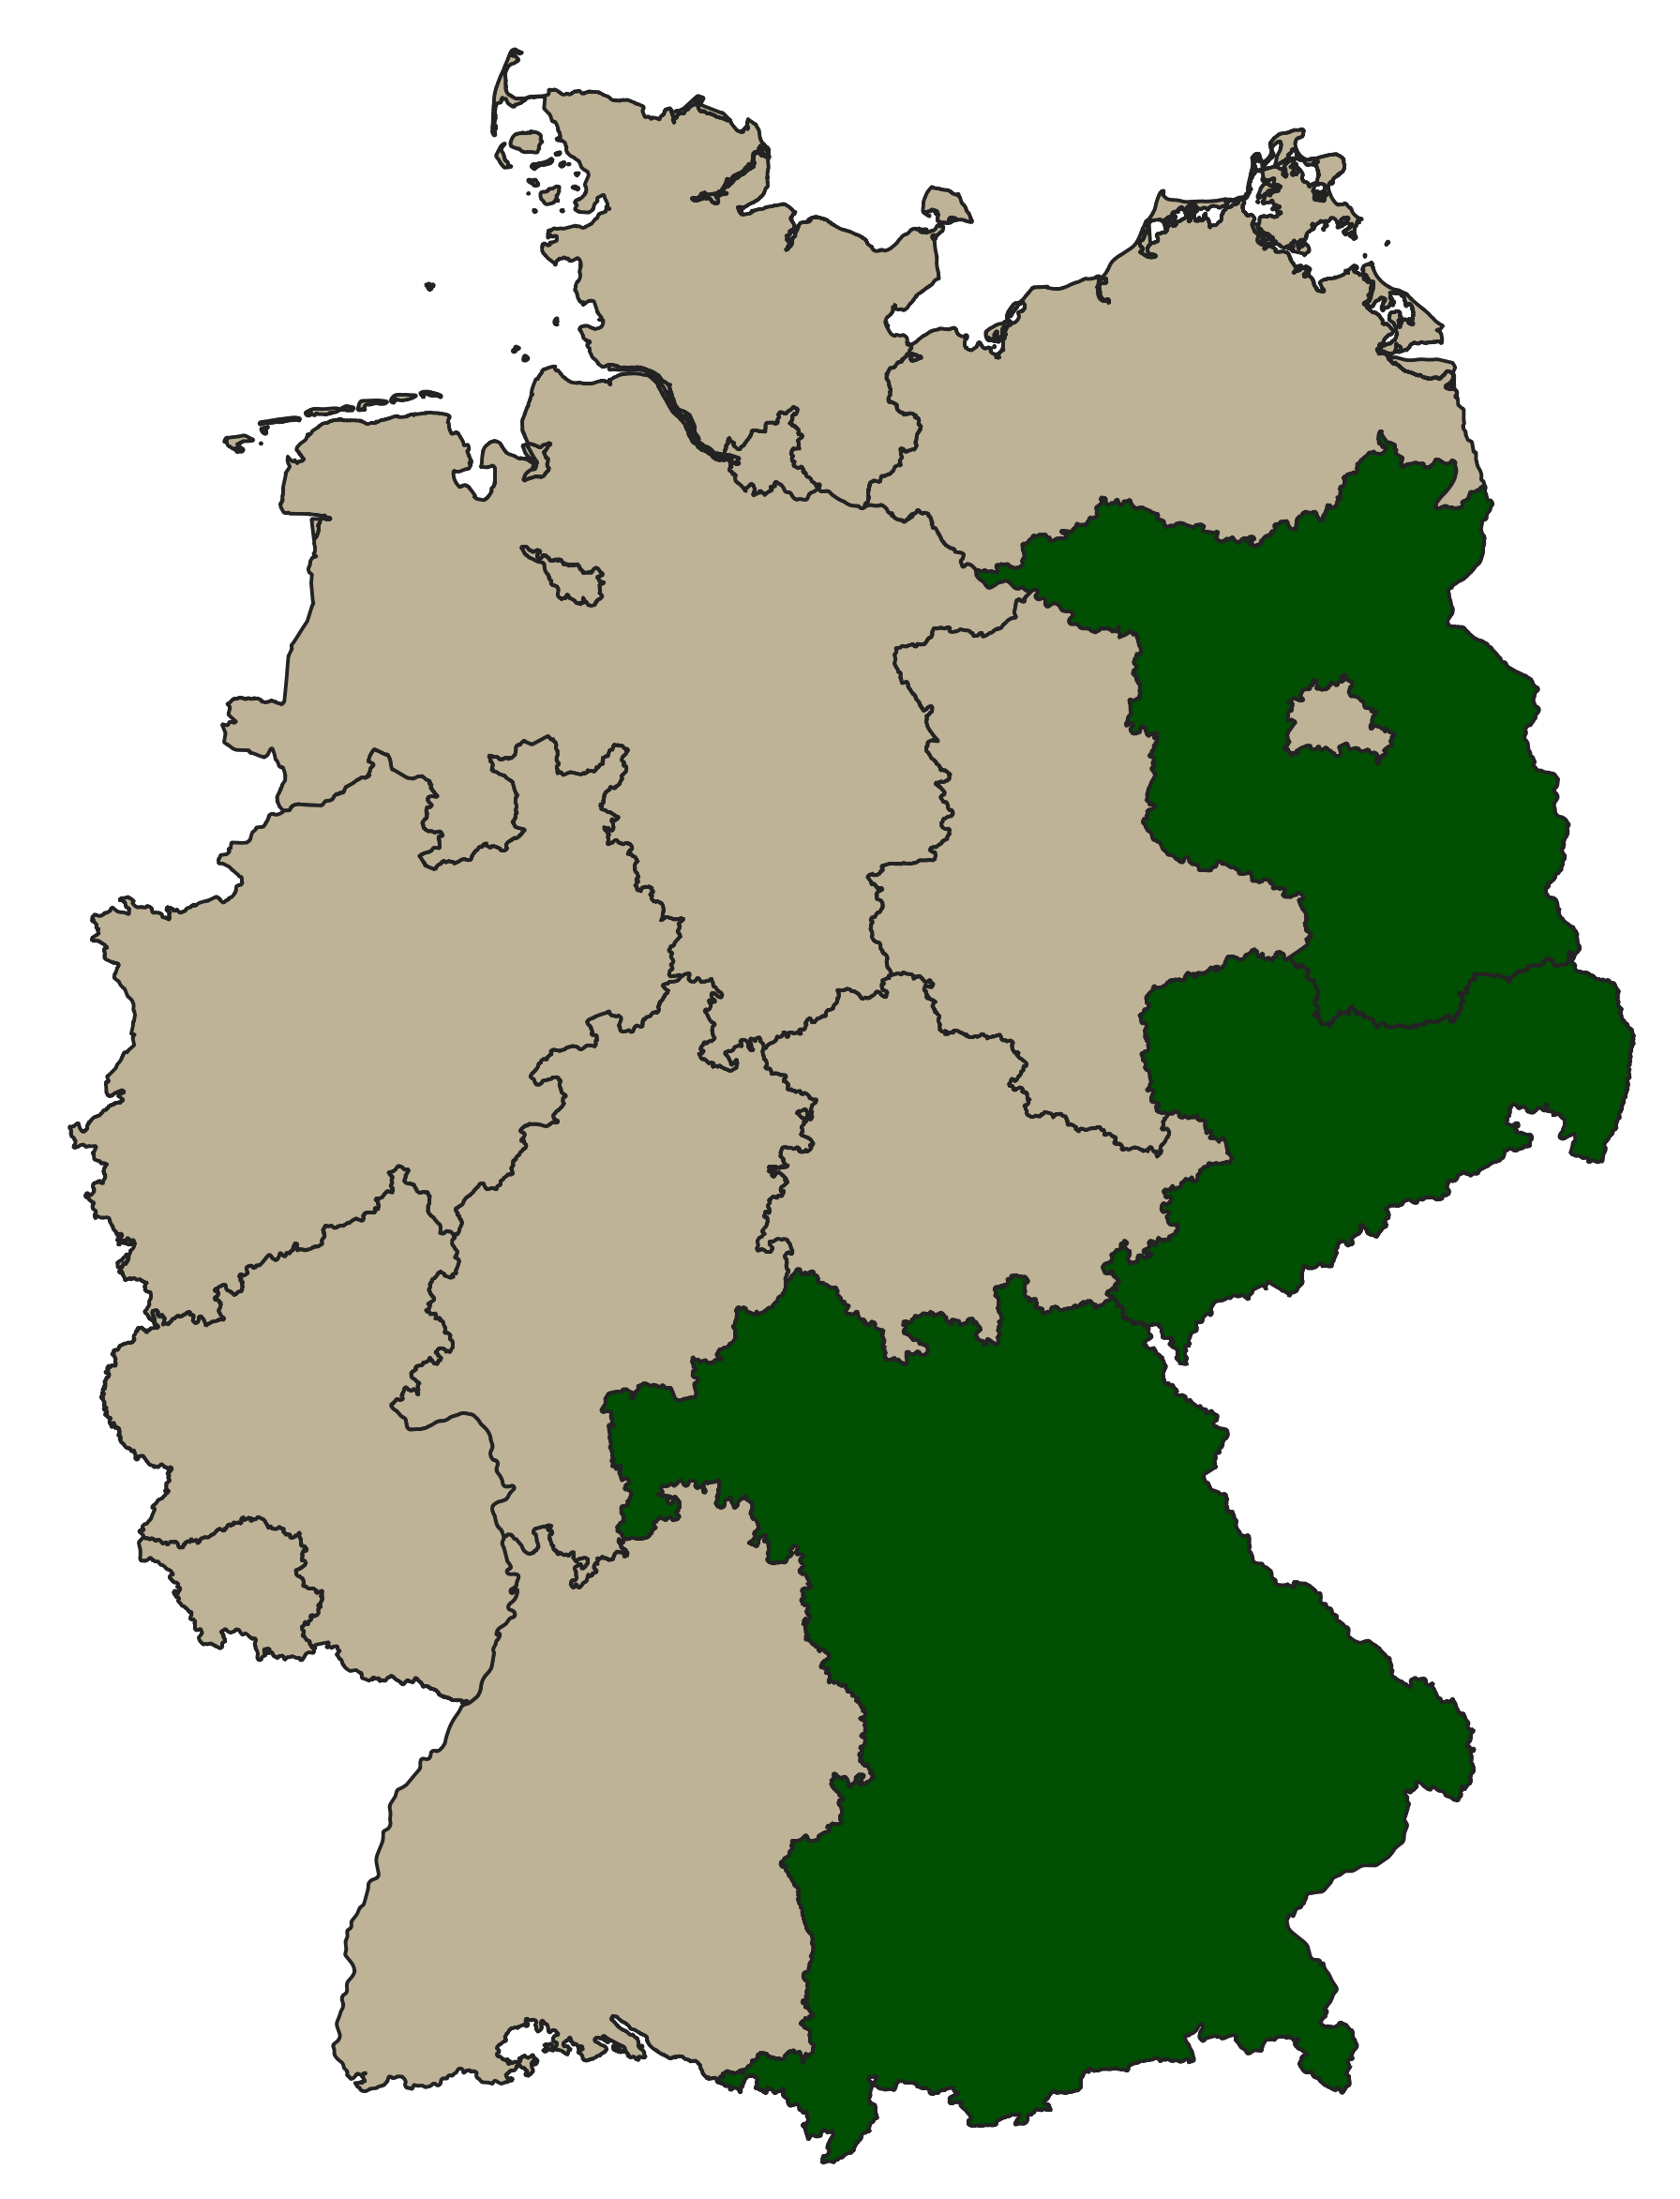
\includegraphics[width=0.5\textwidth]{Mapa_final.png}
	\caption{Distribución de las estaciones climáticas respecto a los estados federados de Alemania. Los polígonos delimitados por un contorno en color negro corresponden a los estados federados reportados por Bundesamt für Kartographie und Geodäsie \cite{States_2025}. En color verde se muestran, de manera descendente, Brandemburgo, Sajonia y Baviera, respectivamente.}
	\label{Stations_per_state}
\end{figure}


Con lo anterior, para cada estado, se obtuvieron un par de calendarios agrícolas: uno empleando la distancia Euclidiana y uno empleando la distancia Manhattan. Lo que permitió la identificación de periodos que favorezcan la siembra, adaptados a las condiciones locales mediante los criterios de decisión previamente establecidos, los cuales se muestran en la Figura \ref{fig:sowing_suitability}

\begin{figure}[htbp]
	\centering
	\begin{tabular}{@{\hspace{-2cm}}c@{\hspace{-0.3cm}}c@{\hspace{-0.3cm}}c@{\hspace{0cm}}c}
		
		% ====================================================
		% Primera fila
		% ====================================================
		
		\begin{subfigure}[b]{0.38\textwidth}
			\centering
			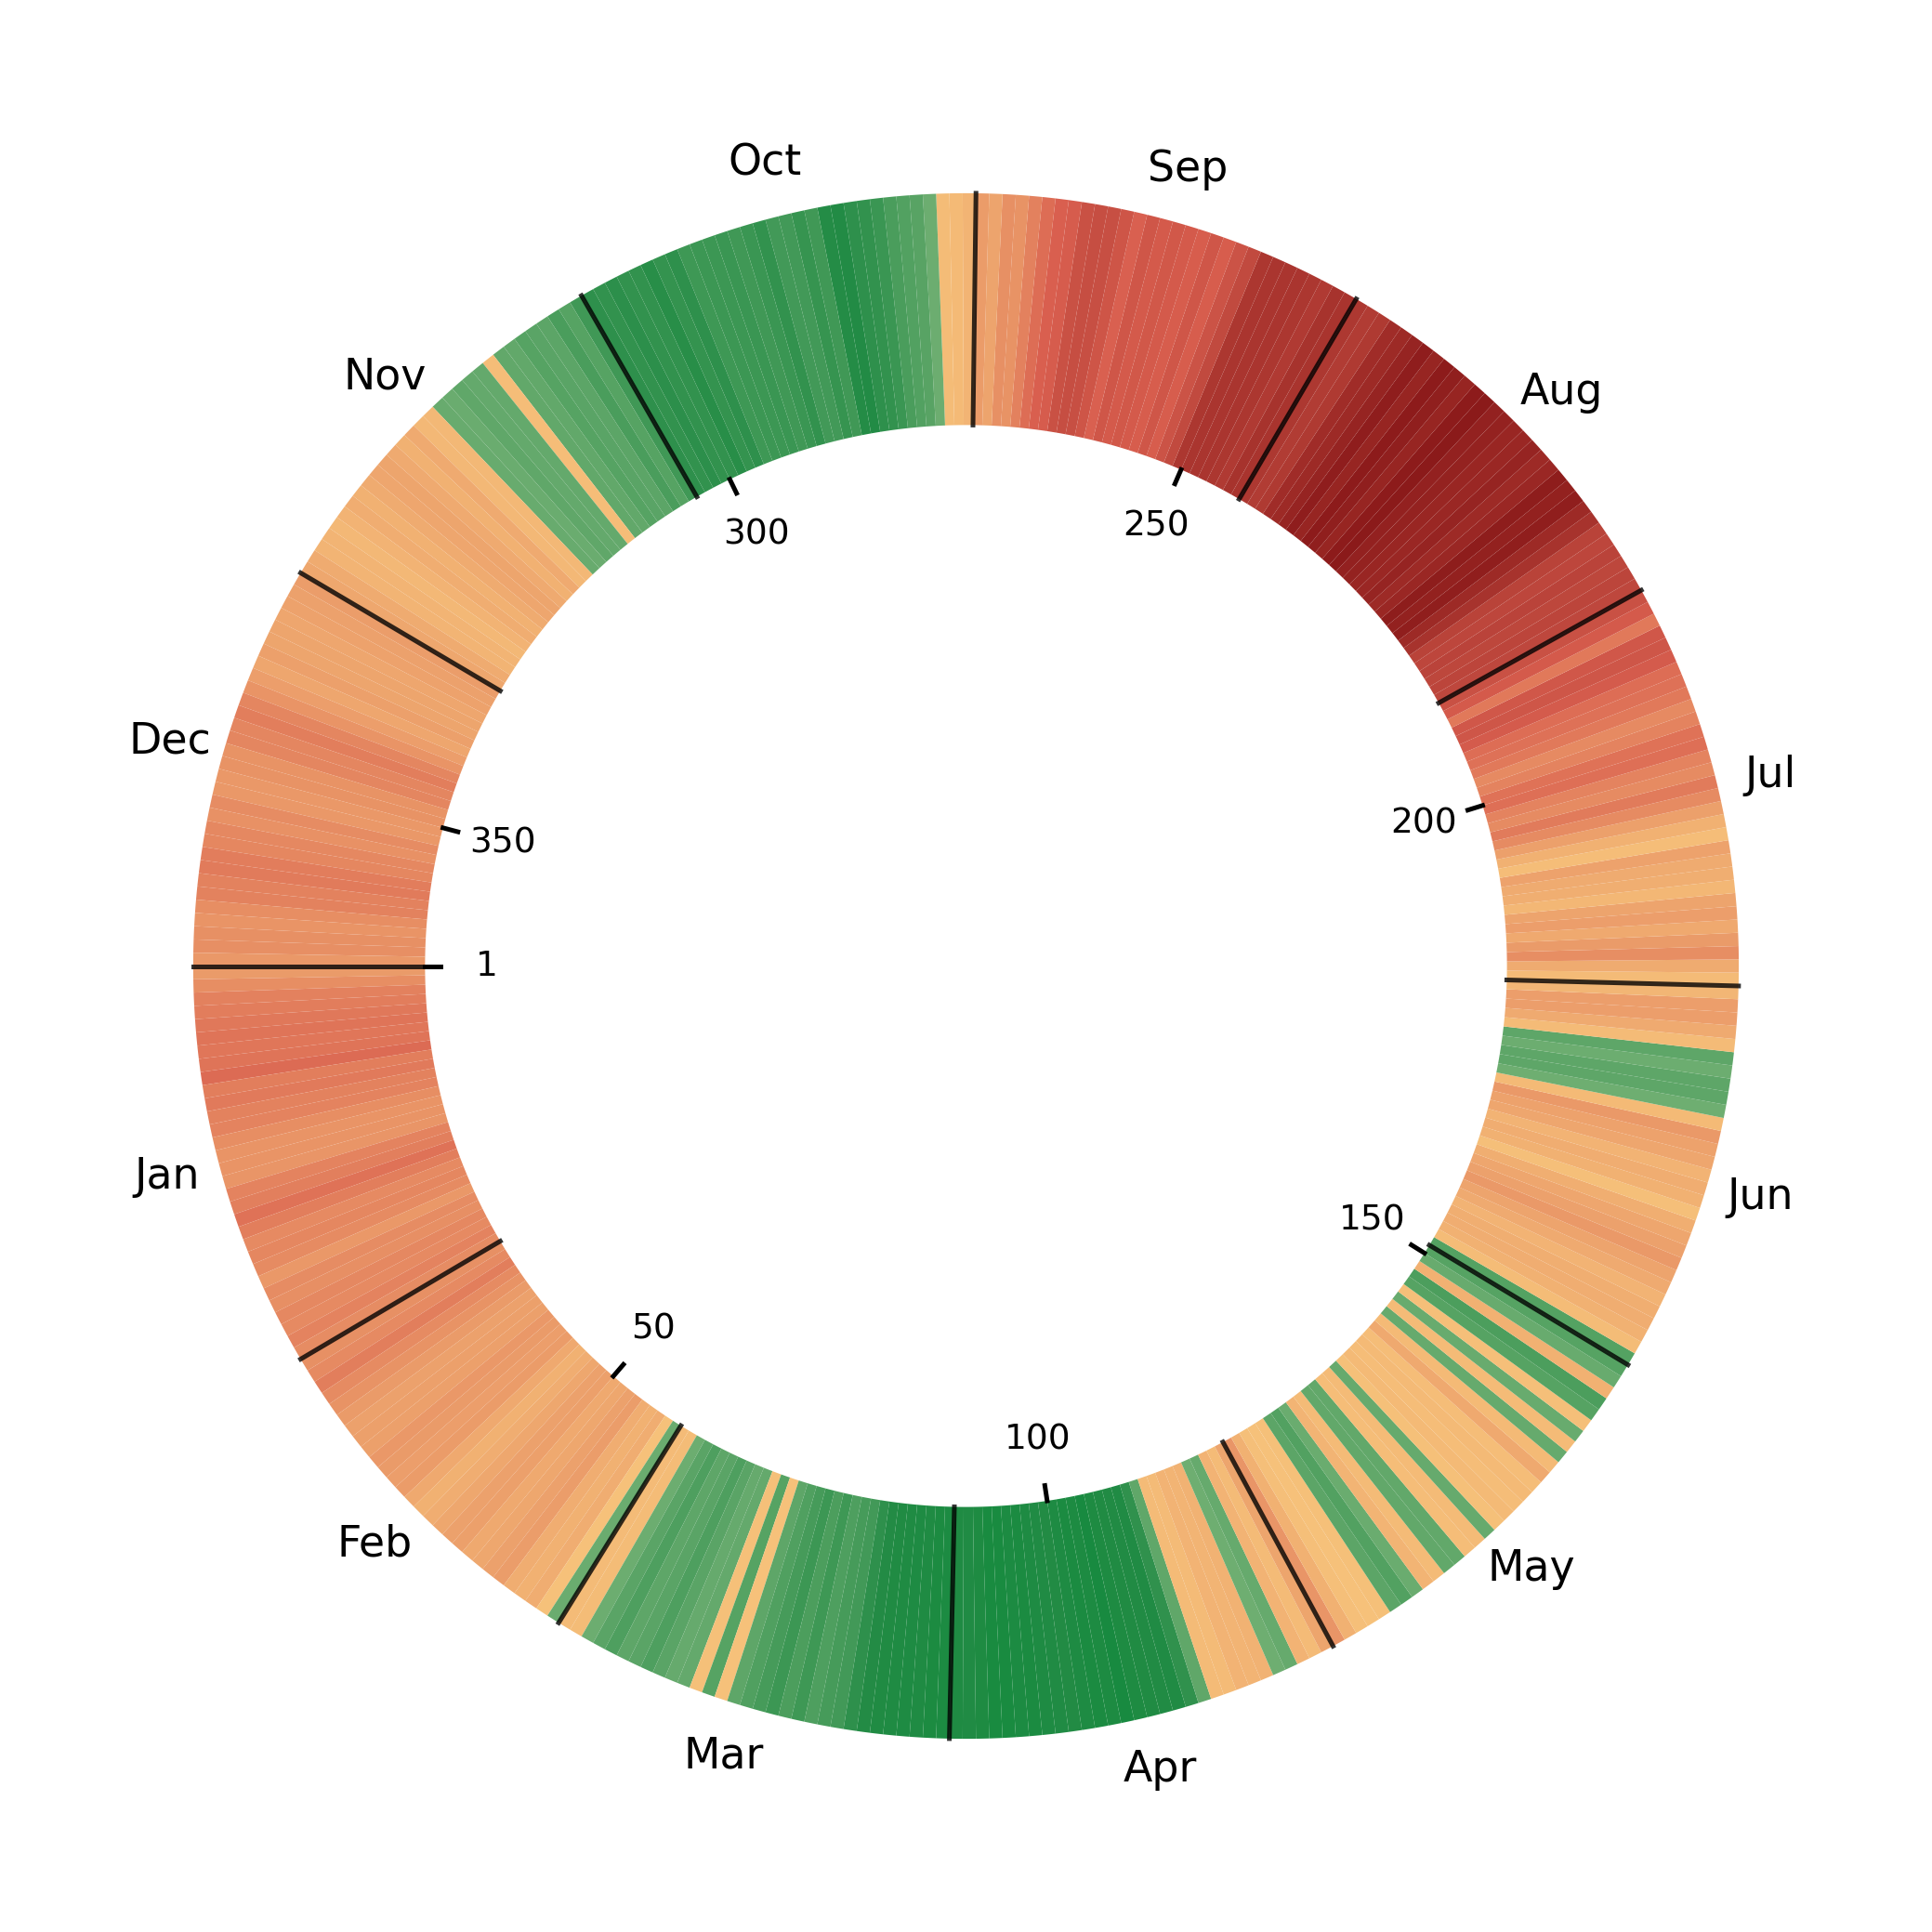
\includegraphics[width=\textwidth]{Brandenburg_Euclidean.png}
			\caption{}
			\label{fig:brandenburg_euclidean}
		\end{subfigure}
		&
		\begin{subfigure}[b]{0.38\textwidth}
			\centering
			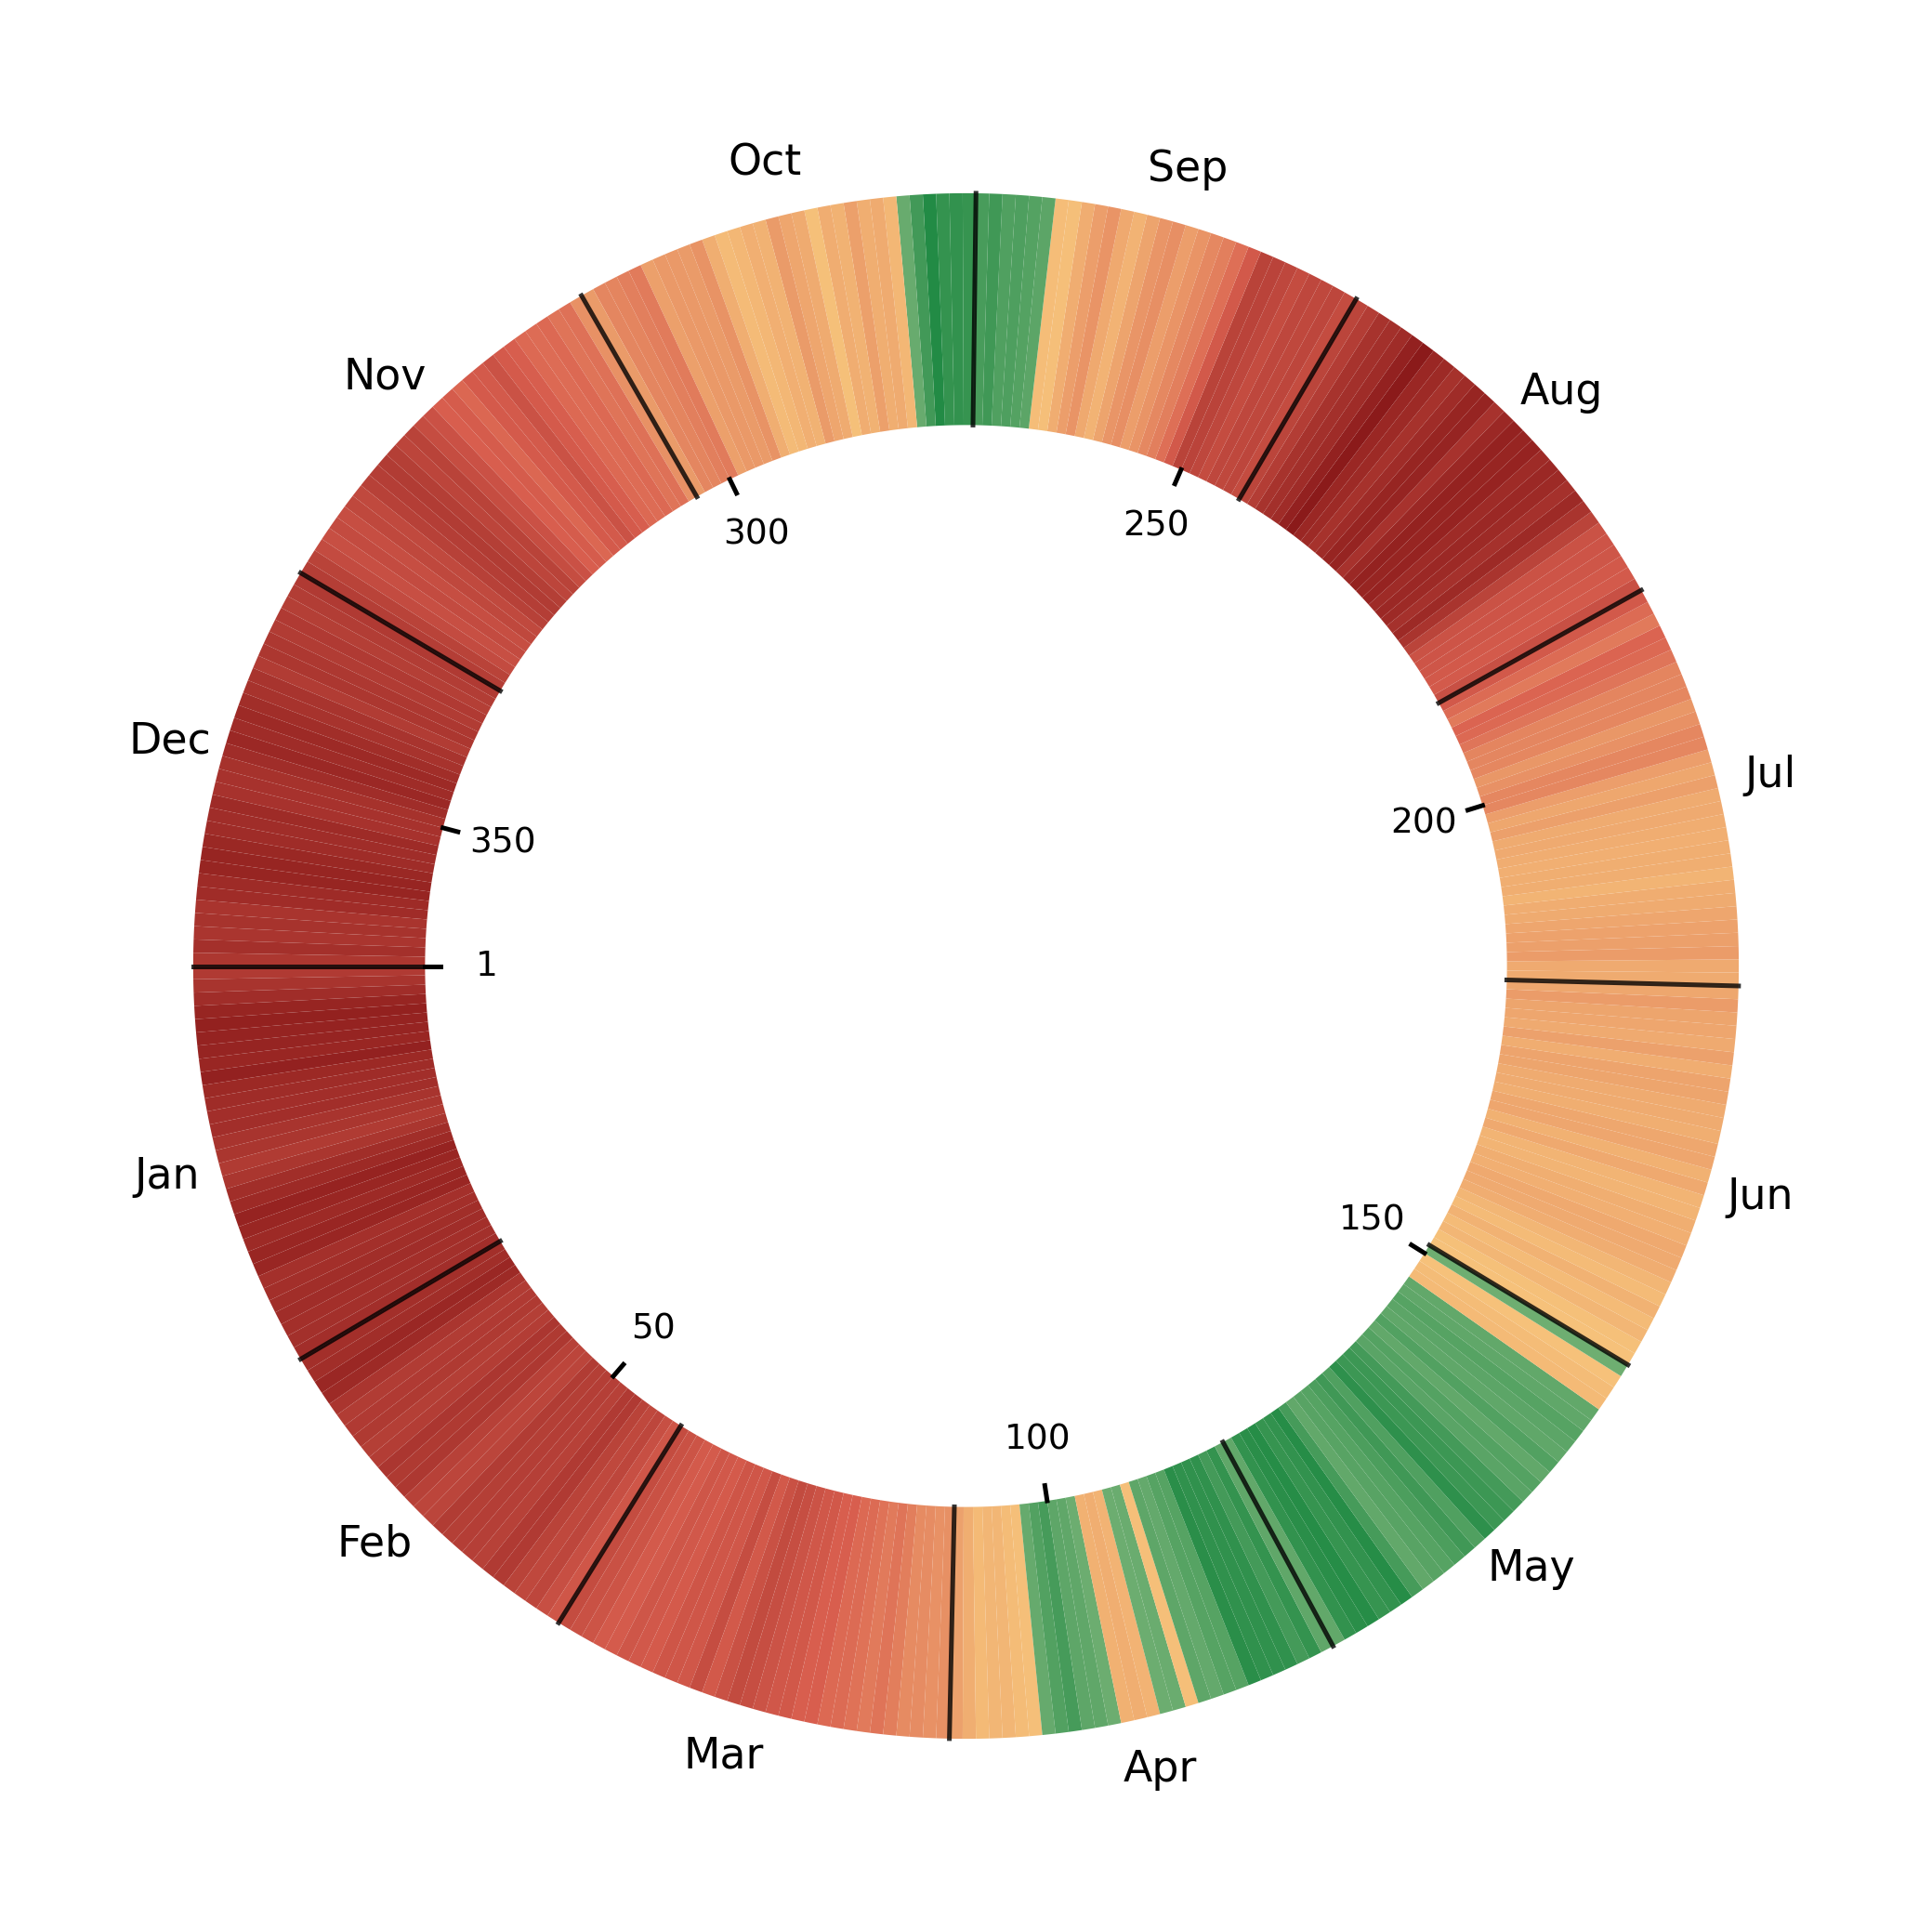
\includegraphics[width=\textwidth]{Saxony_Euclidean.png}
			\caption{}
			\label{fig:saxony_euclidean}
		\end{subfigure}
		&
		\begin{subfigure}[b]{0.38\textwidth}
			\centering
			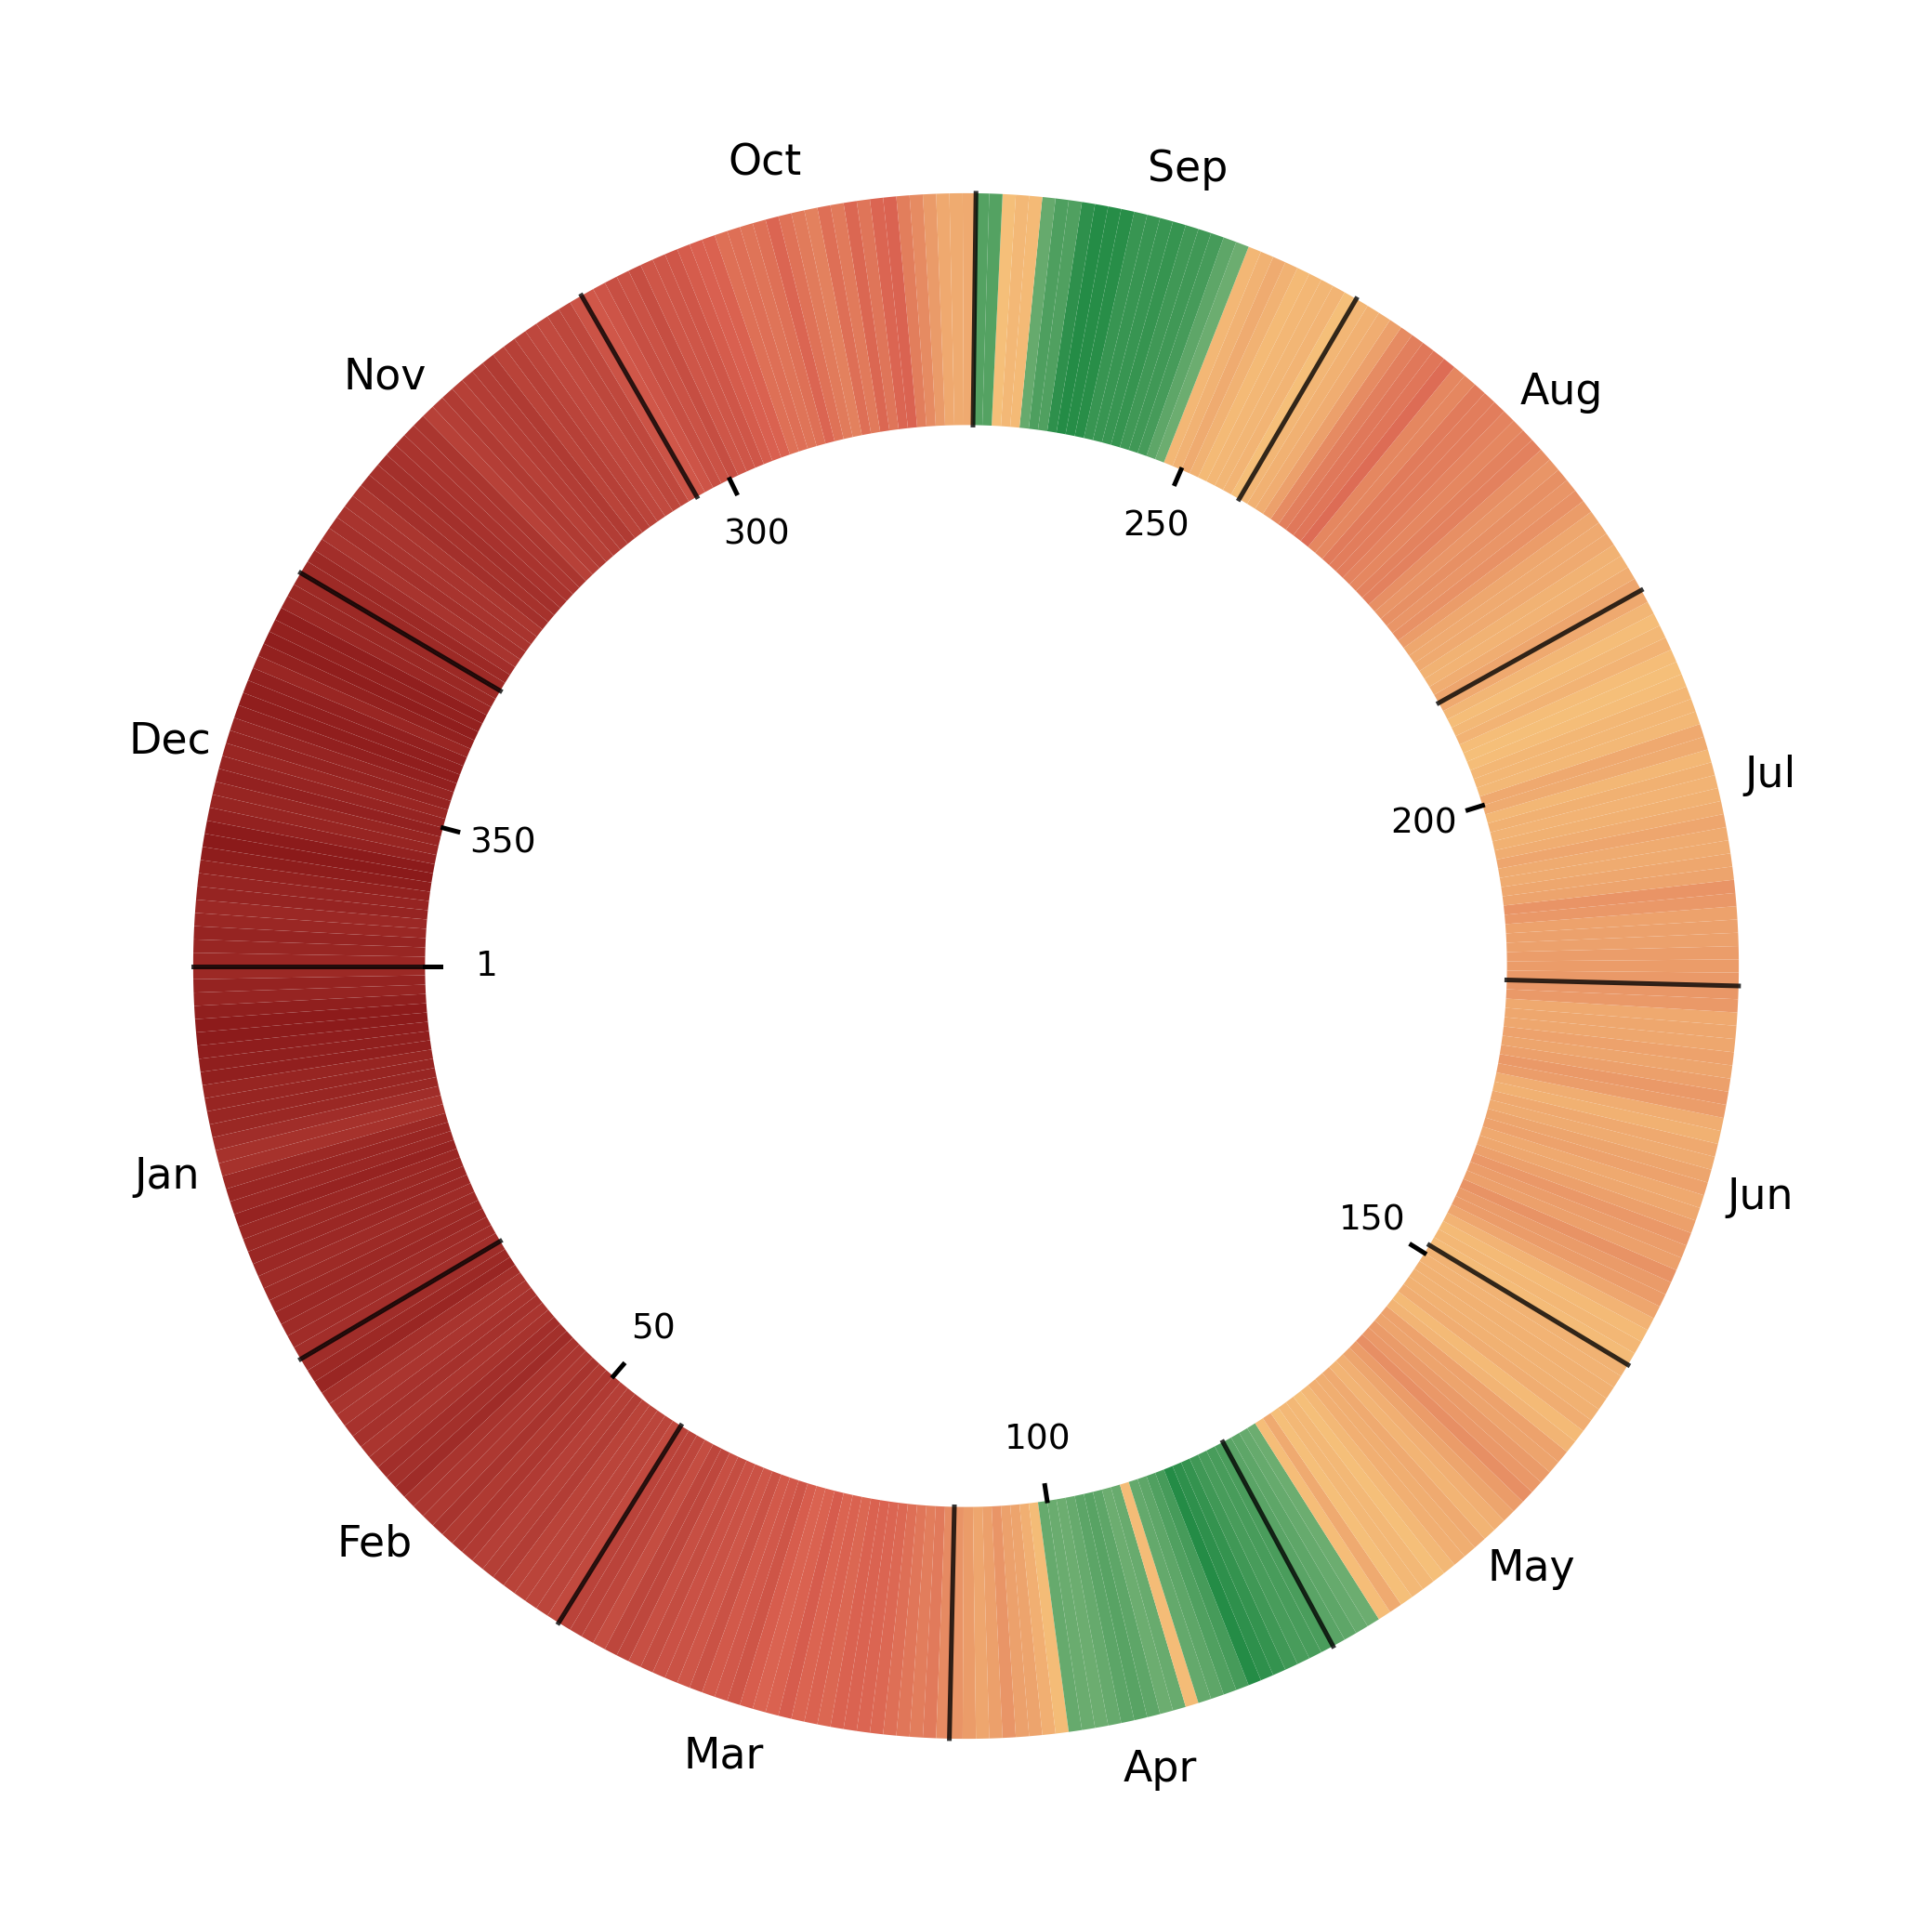
\includegraphics[width=\textwidth]{Babaria_Euclidean.png}
			\caption{}
			\label{fig:bavaria_euclidean}
		\end{subfigure}
		&
		\multirow{2}{*}{
			\begin{subfigure}[t]{0.05\textwidth}
				\centering
				\vspace*{-3.5cm}
				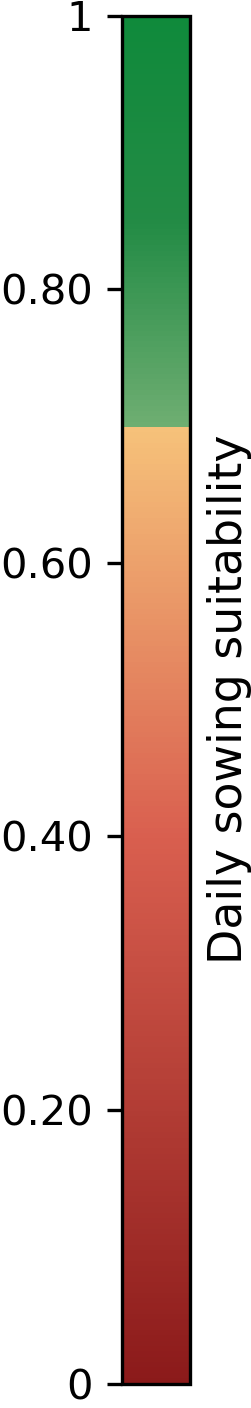
\includegraphics[
				height=0.31\textheight
				]{Suitability.png}
			\end{subfigure}
		}
		\\[2mm]
		
		% ====================================================
		% Segunda fila
		% ====================================================
		
		\begin{subfigure}[b]{0.4\textwidth}
			\centering
			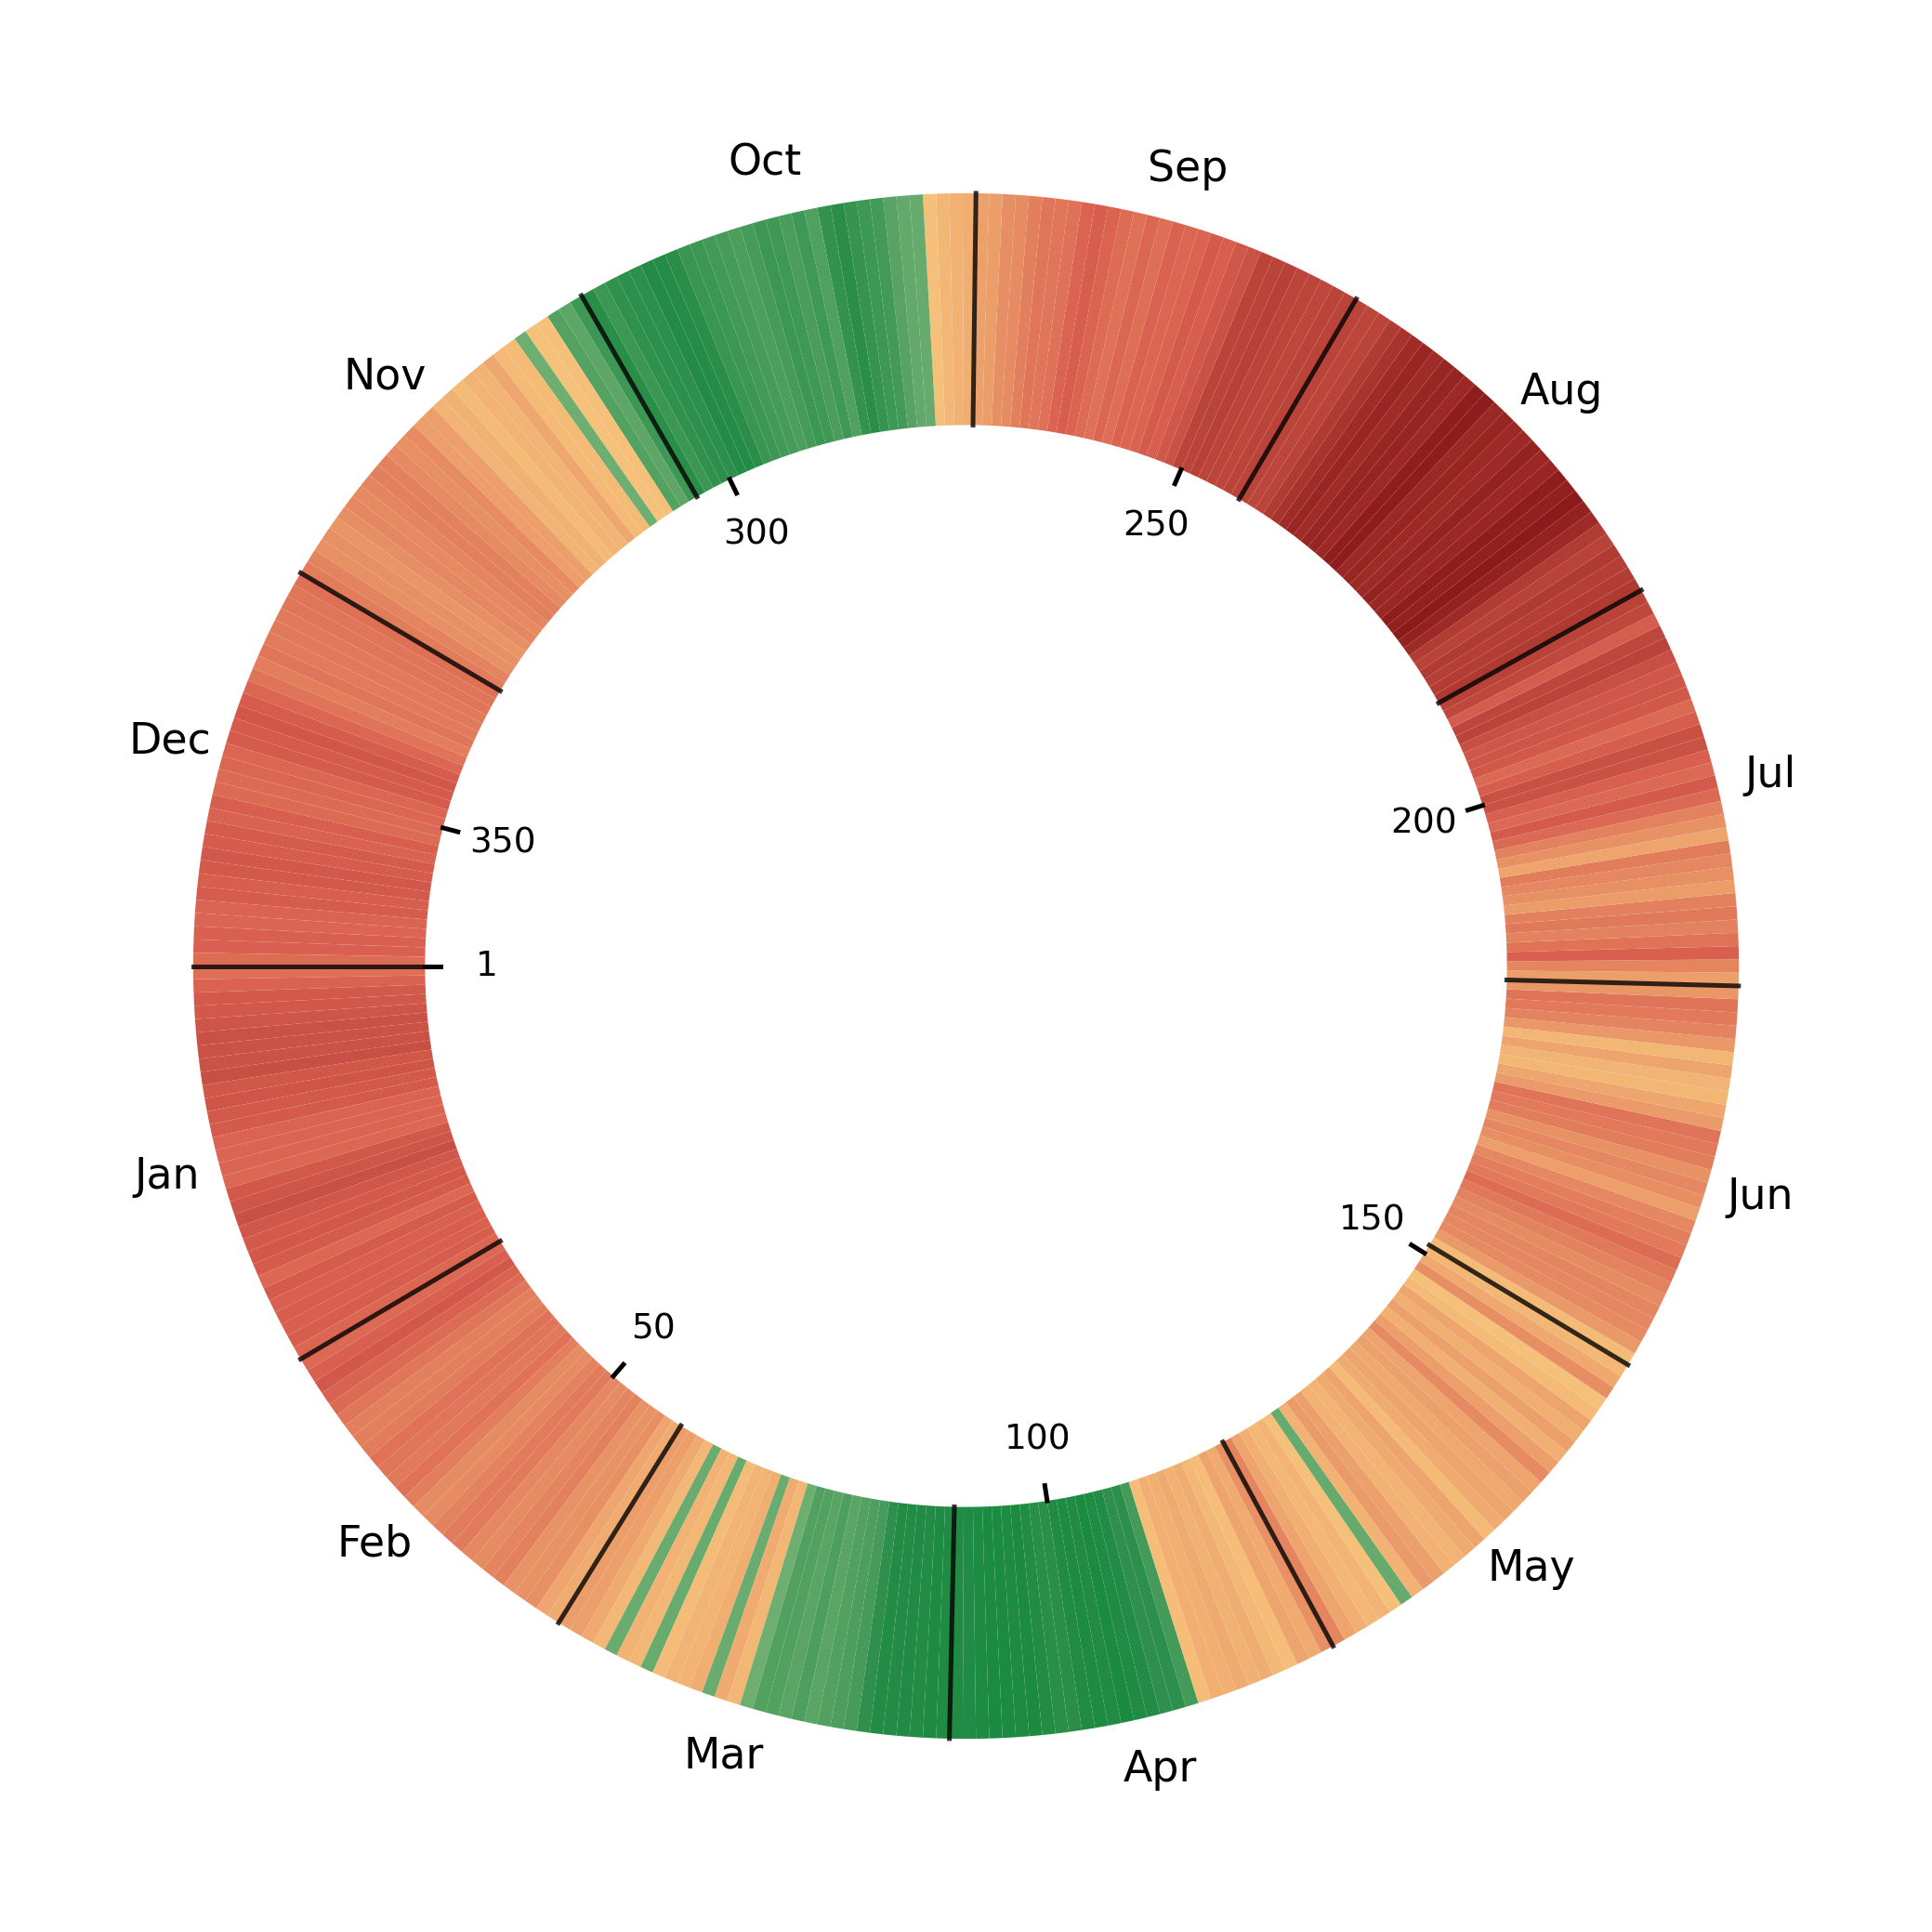
\includegraphics[width=\textwidth]{Brandenburg_Manhattan.png}
			\caption{}
			\label{fig:brandenburg_manhattan}
		\end{subfigure}
		&
		\begin{subfigure}[b]{0.4\textwidth}
			\centering
			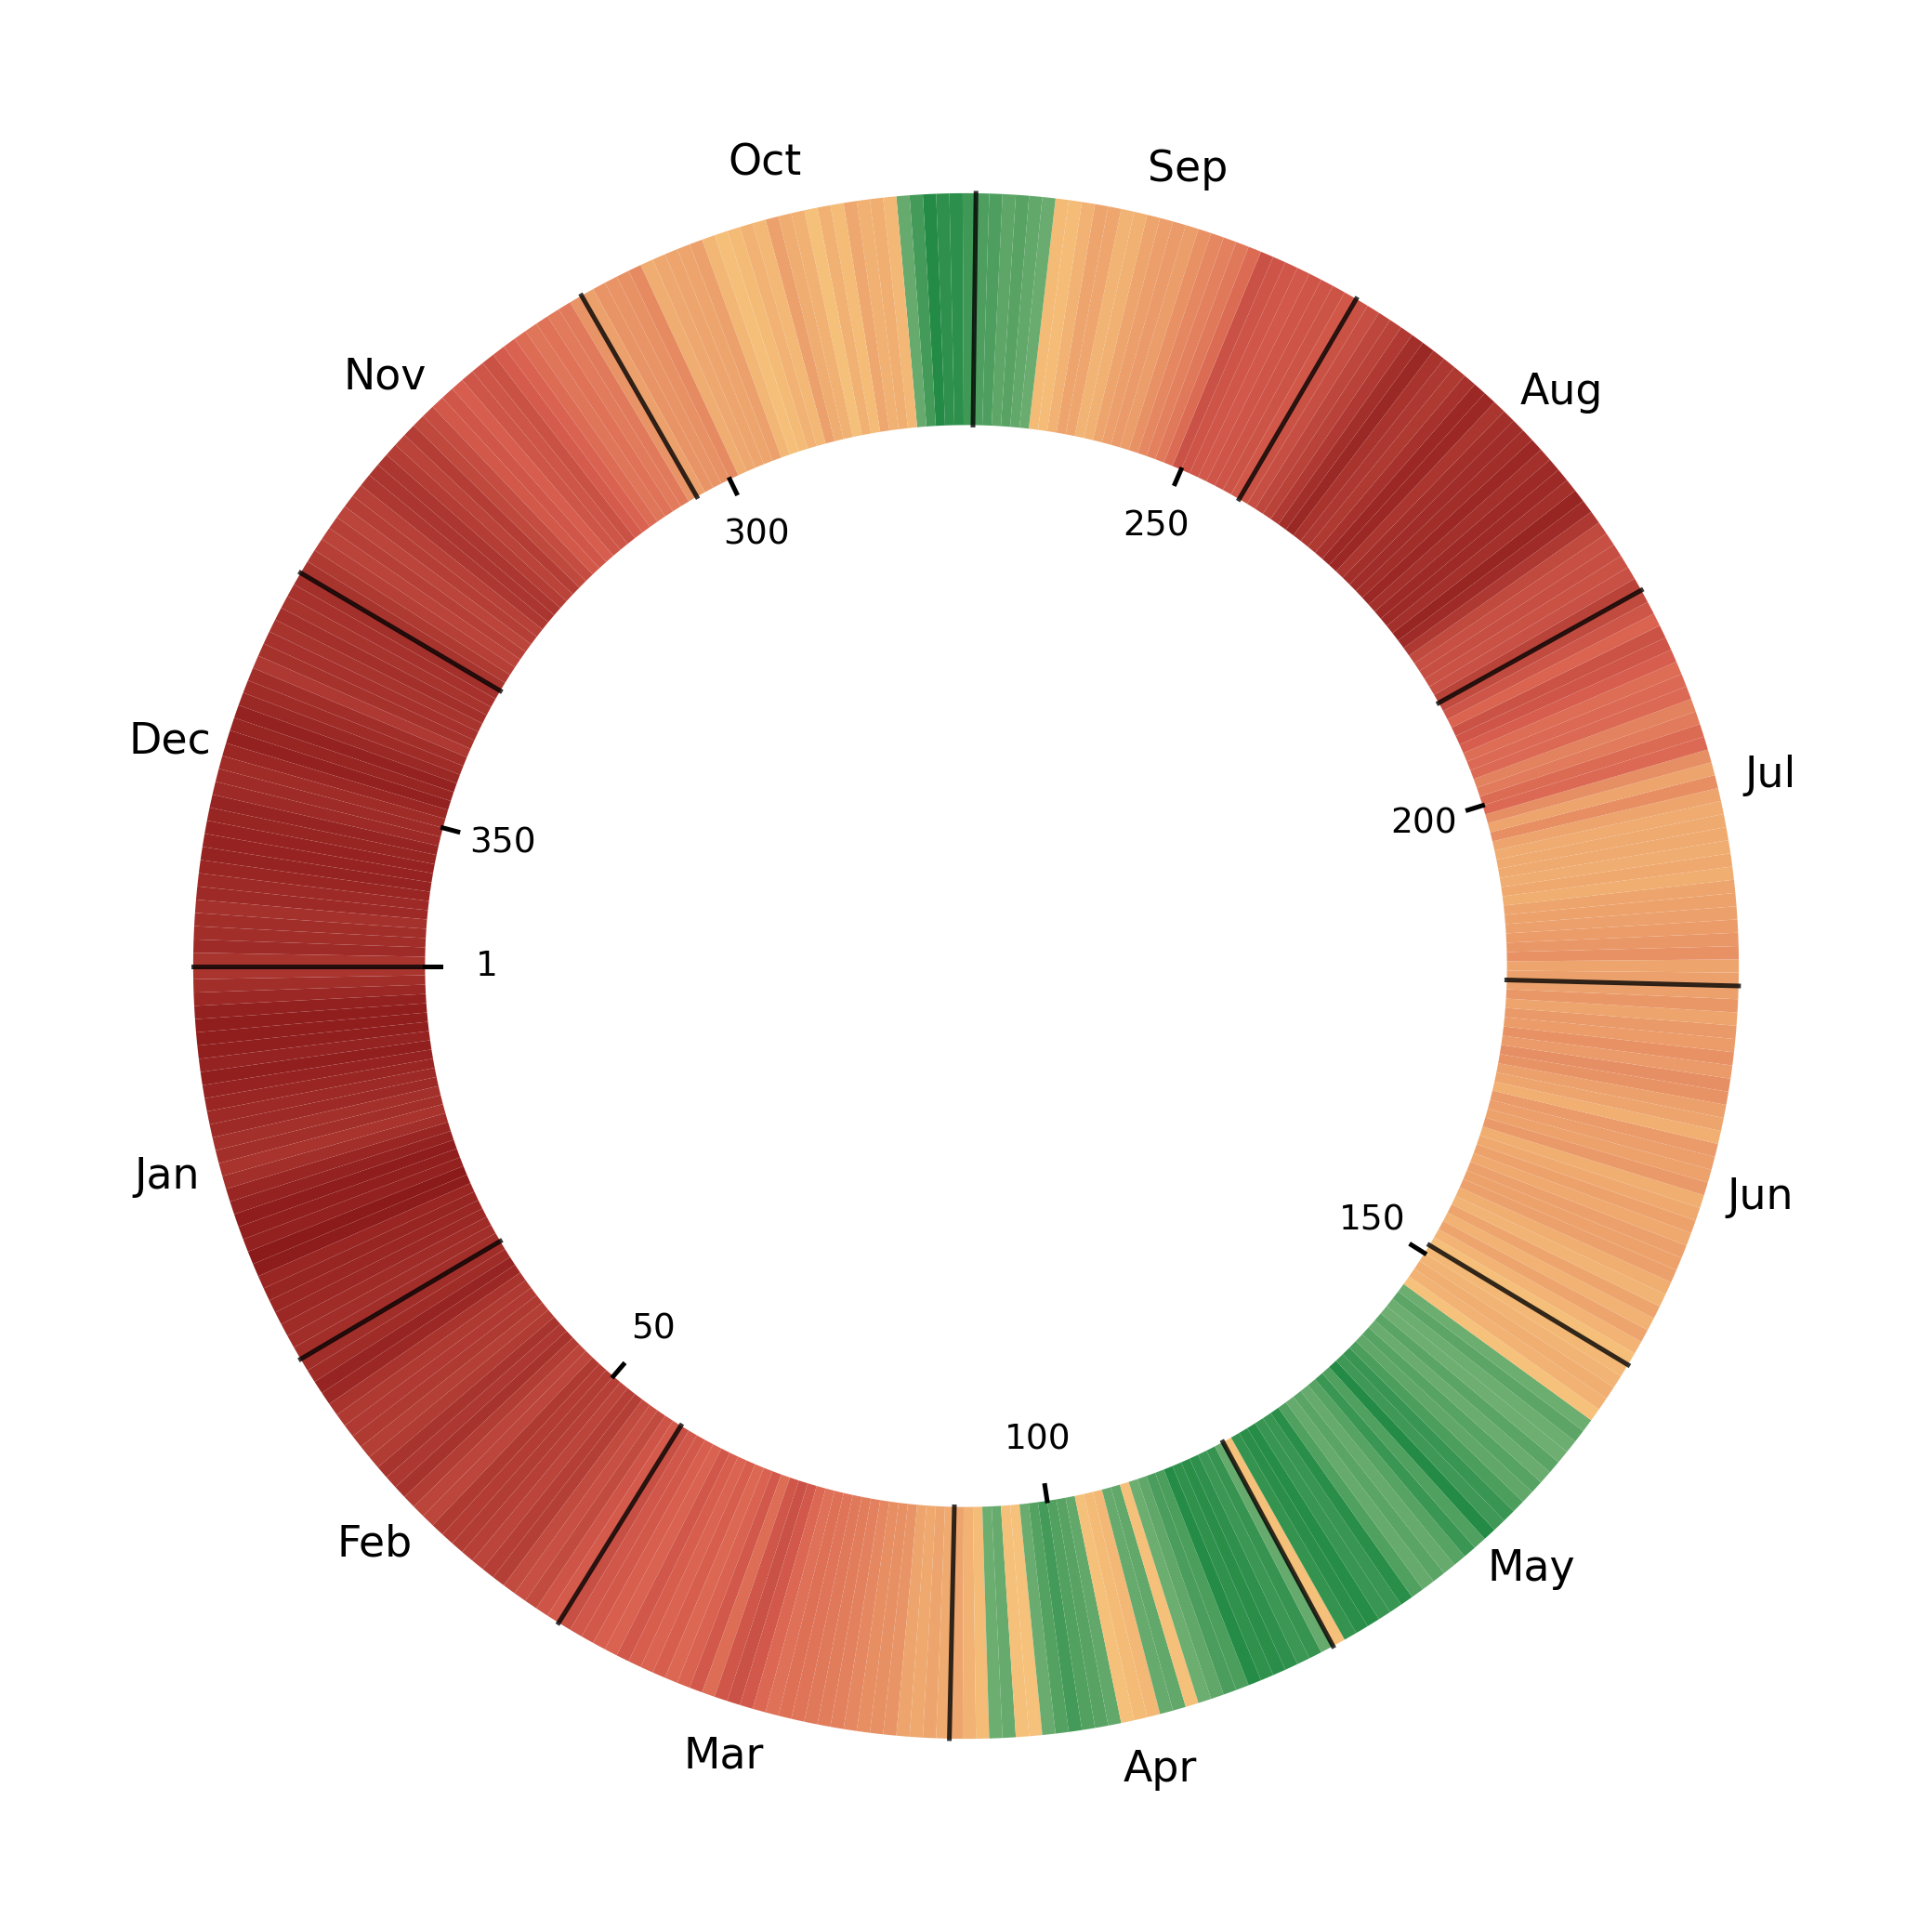
\includegraphics[width=\textwidth]{Saxony_Manhattan.png}
			\caption{}
			\label{fig:saxony_manhattan}
		\end{subfigure}
		&
		\begin{subfigure}[b]{0.4\textwidth}
			\centering
			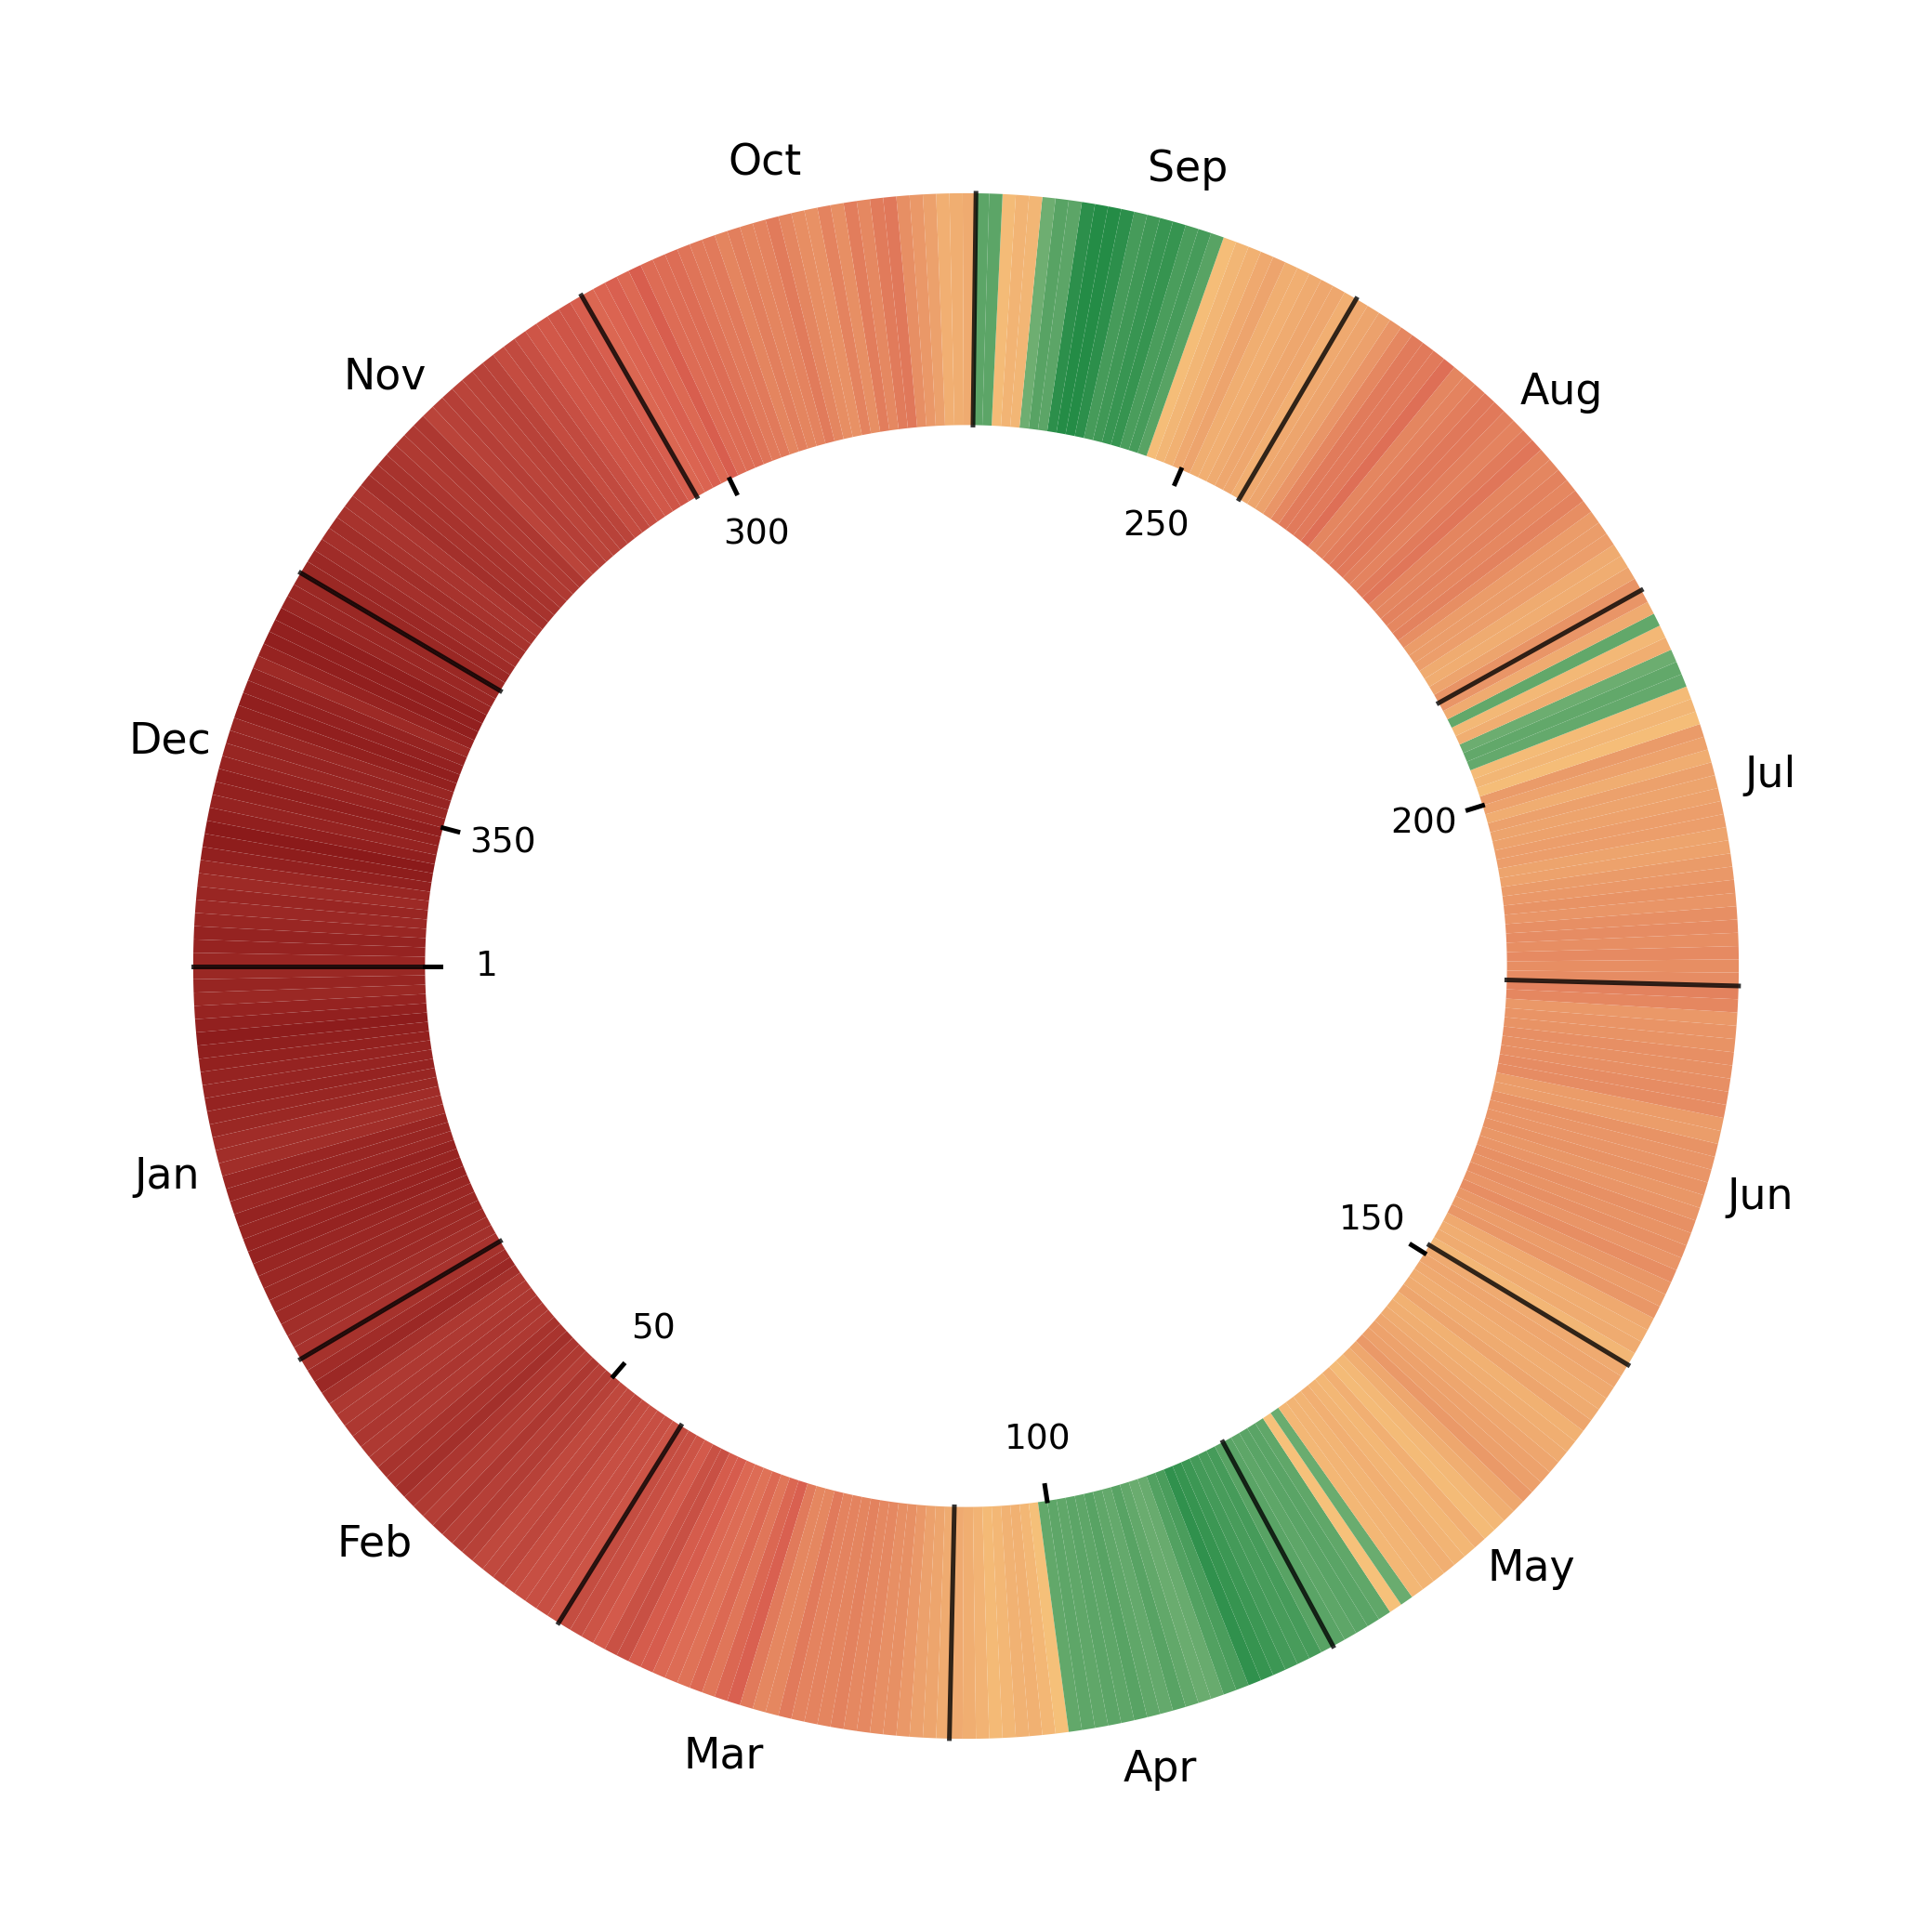
\includegraphics[width=\textwidth]{Babaria_Manhattan.png}
			\caption{}
			\label{fig:bavaria_manhattan}
		\end{subfigure}
		&
		\\
		
	\end{tabular}
	
	\caption{
		Aptitud diaria para la siembra en Brandenburgo, Sajonia y Baviera, expresada como la probabilidad de transición $\lambda_k$, $k\in\{1,2,\ldots,365\}$, calculada mediante las distancias Euclidiana y Manhattan. Las figuras \ref{fig:brandenburg_euclidean}, \ref{fig:saxony_euclidean} y \ref{fig:bavaria_euclidean} muestran los valores de $\lambda_k$ calculados mediante la distancia Euclidiana para Brandenburgo, Sajonia y Baviera, respectivamente. Similarmente, las figuras \ref{fig:brandenburg_manhattan}, \ref{fig:saxony_manhattan} y \ref{fig:bavaria_manhattan} muestran los valores correspondientes calculados mediante la distancia Manhattan. La progresión del año se expresa en sentido contrario a las manecillas del reloj, en el exterior de la gráfica anular se indican los meses, mientras que en su interior se indican los días del año.
	}
	\label{fig:sowing_suitability}
\end{figure}


De acuerdo con \cite{Flores_2025}, la región agrícola empleada se caracteriza por una elevada heterogeneidad topográfica, climática y edáfica. En particular, Baviera, Brandemburgo y Sajonia presentan variaciones en humedad, altitud, temperatura y características del suelo, factores que influyen directamente en las prácticas agrícolas y los calendarios de siembra. Esta diversidad de condiciones ambientales permitió someter la metodología propuesta a distintos escenarios espaciales y verifica su capacidad para identificar variaciones en la aptitud de las fechas de siembra y, con ello, evaluar parcialmente su comportamiento bajo condiciones ambientales heterogéneas.\\


\section{Cronograma de actividades}



Durante el semestre en curso se contempla emplear los datos correspondientes a las fechas de siembra de maíz en Alemania, reportados por \citet[Tabla 1]{Parker_2016}, a partir de los criterios topográficos y geográficos descritos por \cite{Flores_2025}, ver Tabla \ref{Real_data}. Los cuales, tras identificar una métrica apropiada, sirvan para realizar una comparación complementaria con resultados previamente publicados.\\

\begin{table}[h]
	\centering
	\begin{tabular}{l|c|c}
		\hline
		\multicolumn{1}{c|}{\textbf{Región}} & \textbf{Características} & \textbf{Fecha de siembra} \\ \hline
		
		\multirow{3}{*}{\parbox{4.5cm}{\textbf{Brandemburgo}\\ \textbf{Norte de Sajonia}}} 
		& Altitud menor que $250$ m.s.n.m. 
		& $115.6 \pm 7.12$ \\ \cline{2-3}
		
		
		& Latitud mayor o igual que $51^\circ$ N. 
		& $116.2 \pm 7.08$ \\ \cline{2-3}
		
		& Longitud mayor o igual que $8.5^\circ$ E. 
		& $116.2 \pm 7.3$ \\ \hline
		
		
		\multirow{3}{*}{\parbox{4.5cm}{\textbf{Sur de Sajonia}\\ \textbf{Baviera}}}  
		& Altitud mayor o igual que $250$ m.s.n.m. 
		& $117.4 \pm 8.29$ \\ \cline{2-3}
		
		
		& Latitud menor que $51^\circ$ N. 
		& $116.7 \pm 8.23$ \\ \cline{2-3}
		
		& Longitud mayor o igual que $8.5^\circ$ E. 
		& $116.2 \pm 7.3$ \\ \hline
		
	\end{tabular}
	\caption{Fechas promedio de siembra de maíz y sus correspondientes desviaciones estándar reportadas por \cite{Parker_2016}, asociadas a las características geográficas y topográficas descritas por \cite{Flores_2025} para Brandemburgo, Sajonia y Baviera.}
	\label{Real_data}
\end{table}


Adicionalmente, se llevará a cabo la construcción de los intervalos de confianza correspondientes mediante los métodos de bootstrap y jackknife, así como la integración de los resultados restantes en la redacción del artículo. Finalmente, se contempla la presentación de los avances y resultados en el Congreso Internacional de Ecología Estadística (ISEC, por sus siglas en inglés), que se llevará a cabo del 10 al 15 de enero de 2027 en Mérida, México.



\begin{figure}[h]
	\resizebox{\linewidth}{!}{%
		\centering
		\begin{ganttchart}[
			hgrid,
			vgrid,
			x unit=1.8cm,
			y unit chart=0.7cm,
			bar height=0.5,
			group height=0.7,
			title height=1,
			milestone height=.6,
			bar/.style={fill=blue!50},
			group/.style={fill=gray!50},
			title/.style={fill=gray!20},
			milestone/.style={fill=red},
			bar label font=\small,
			group label font=\bfseries\small
			]{1}{6}
			
			% -------------------------------------------------
			% ENCABEZADOS
			% -------------------------------------------------
			
			\gantttitle{Cronograma de actividades}{6} \\
			
			\gantttitle{Ago. 2026}{1}
			\gantttitle{Sept 2026}{1}
			\gantttitle{Oct 2026}{1}
			\gantttitle{Nov 2026}{1}
			\gantttitle{Dic. 2026}{1}
			\gantttitle{Ene. 2027}{1}
			\\
			
			% -------------------------------------------------
			% ANÁLISIS DE DATOS
			% -------------------------------------------------
			
			\ganttgroup{Análisis de datos y comparación}{1}{5} \\

			\ganttbar
			{Identificación de una métrica apropiada}
			{2}{3} \\
			
			\ganttbar
			{Comparación con resultados previamente publicados}
			{3}{5} \\
			
			% -------------------------------------------------
			% INTERVALOS DE CONFIANZA
			% -------------------------------------------------
			
			\ganttgroup{Construcción de intervalos de confianza}{1}{2} \\
			
			\ganttbar
			{Bootstrap}
			{1}{2} \\
			
			\ganttbar
			{Jackknife}
			{1}{2} \\
			
			% -------------------------------------------------
			% PRODUCCIÓN CIENTÍFICA
			% -------------------------------------------------
			
			\ganttgroup{Integración y redacción científica}{4}{5} \\
			
			\ganttbar
			{Integración de resultados en el artículo}
			{4}{5} \\
			
			% -------------------------------------------------
			% PRESENTACIÓN
			% -------------------------------------------------
			
			\ganttgroup{Presentación de resultados}{5}{6} \\
			
			\ganttbar
			{Preparación de resultados para el ISEC}
			{5}{5} \\
			
			\ganttmilestone
			{ISEC 2027}
			{6}
			
		\end{ganttchart}
		
	} % fin resizebox
	
	\caption{Cronograma de actividades correspondientes al semestre agosto--diciembre de 2026.}
	\label{fig:gantt_semestre}
	
\end{figure}
		
		\iffalse
		{\color{black}
			A Results section is expected for all experimental work; although, depending on the Methods section, an alternative
			Results section heading might be more appropriate. \ Results should be clear and concise; and report only your work,
			i.e., comparisons with others$\text{\textgreek{’}}$ works from cited literature should be set out in the subsequent
			section, Discussion. \ A combined Results and Discussion section may be appropriate, but if this is adopted, it is
			essential to maintain clarity regarding which results/achievements are your work and which are the work of others.
			\ Because detailed results often appear in tables and figures, there is no need to duplicate specific values in the
			text of the paper$\text{\textgreek{—}}$except, perhaps, for emphasis or to provide interpretation or elaboration. \ }
		
		{\color{black}
			Numerical results provide objective evidence related to the outcomes of reported research. \ However, such experimental
			outcomes always involve some randomness and so produce ranges of values. \ Statistical analyses are the only way to
			distinguish such randomness from meaningful responses that can support the study$\text{\textgreek{’}}$s conclusions.}
		\fi
		
		\bigskip
		
		%\section{Discussion}
		\iffalse
		{\color{black}
			The Discussion section should organize, interpret, and evaluate the study$\text{\textgreek{’}}$s results. \ Discussion
			(interpretation/evaluation) properly positions the obtained results within the context of the problem, practical
			considerations, and limitations of the study. \ It is recommended to compare and contrast the current results to those
			results reported by others.}
		\fi
		
		\bigskip
		
		
		%\section{Conclusions}
		%The period from planting to emergence depends on soil temperature, soil moisture, soil aeration, and seed vigor
		% See: https://acsess.onlinelibrary.wiley.com/doi/abs/10.2134/agronmonogr18.3ed.c10
		
		\iffalse
		{\color{black}
			As noted above, the Conclusions section should \textit{not} summarize the paper$\text{\textgreek{’}}$s contents; neither
			should it reiterate methods and results. \ A Conclusions section should succinctly present the research study's
			findings (What did we learn? What new knowledge has been uncovered? How has the state of the art been advanced? What
			new research directions or studies are suggested by the current findings?). \ Bulleted or numbered lists should be
			avoided, as concluding statements most often require additional explanation to properly condition their applicability
			or relevance. \ This section stands as the most important part of the paper, as it establishes the significance of the
			work reported.}
		\fi
		
		\bigskip
		\newpage
		\section{Revistas}
		El proyecto en desarrollo presenta tanto una metodología matemática nueva en el área de predicción fenológica como resultados con potencial impacto en el campo agrícola, dado que se trata de un calendario agrícola basado en un modelo de autoría propia. Por tanto, para la publicación del trabajo como un artículo de investigación en una revista científica se han considerado aquellas revistas cuyos alcances, objetivos y publicaciones previas sean compatibles con el balance entre un desarrollo metodológico teórico y un análisis bajo condiciones reales.\\

Con lo anterior y con base en la literatura consultada hasta el momento, en la siguiente tabla se presentan las revistas indexadas propuestas para someter nuestro trabajo en el mediano plazo.\\


\begin{table}[h]
	\centering
	\begin{tabular}{p{7.5cm}|c|c}
		\hline
		\textbf{Revista} & \textbf{Factor de impacto} & \textbf{Referencias consultadas} \\
		\hline
		\href{https://www.sciencedirect.com/journal/computers-and-electronics-in-agriculture/about/aims-and-scope}{Computers and Electronics in Agriculture}\newline
		Editorial: Elsevier B.V.
		& 10.3
		& \cite{Elnesr_2013} \\ \hline
		\href{https://www.sciencedirect.com/journal/sustainable-computing-informatics-and-systems}{Sustainable Computing: Informatics and Systems}\newline
		Editorial: Elsevier B.V.
		& 6.2
		& \cite{GUMUSCU2020100308} \\ \hline
		\href{https://onlinelibrary.wiley.com/journal/1439037x}{Journal of Agronomy and Crop Science}\newline
		Editorial: Wiley.
		& 3.2
		& \cite{Parker_2016} \\ 
		\hline
	\end{tabular}
	\caption{Revistas idexadas en el Journal Citation Reports (JCR)   consideradas para la publicación del artículo, factor de impacto y las referencias relacionadas con el proyecto consultadas en ellas.}
	\label{tab:journals}
\end{table}


Derivado del avance obtenido y considerando las actividades pendientes de programación, redacción y revisión, se propone diciembre de 2027 como fecha tentativa para el envío del manuscrito a una de las revistas antes mencionadas, correspondiendo con el final del quinto semestre del doctorado.

		
		
		%\textbf{\textcolor{black}{Acknowledgements}}
		
		\iffalse
		{\color{black}
			Collate acknowledgements in a separate section at the end of the article before the references and do not, therefore,
			include them on the title page, as a footnote to the title or otherwise. \ List here those individuals who provided
			help during the research (e.g., providing language help, writing/reviewing assistance, collecting and/or organizing
			data, funding assistance, project administration, supervision, or proof reading, etc.). \ Only those individuals, who
			provided substantive and essential intellectual/scientific contributions, should be listed as authors;
			others$\text{\textgreek{’}}$ contributions should be acknowledged here.}
		\fi
		
		\bigskip
		
		
		\bigskip
		
		\clearpage{}
		\bibliographystyle{plainnat} 
		\bibliography{PaperBibliography}
		\iffalse
		{\color{black}
			All publications cited in the text should be presented in a list of references following the text of the manuscript.
			\ The manuscript should be carefully checked to ensure that the spelling of authors$\text{\textgreek{’}}$ names and
			dates are the same in the text as in the reference list.}
		
		{\color{black}
			The journal uses an author-date format for literature citations and a correspondingly alphabetized list of references.}
		
		{\color{black}
			Typically, for a non-Review Article, 25-35 key or seminal references are sufficient. \ Readers can readily find
			subsequent literature using Scopus and Internet search engines.}
		
		{\color{black}
			In the text refer to the author's surname (without initials) and year of publication, followed - if necessary - by a
			short reference to appropriate pages. \ Examples: {\textquotedbl}Since Peterson (1993) has shown that
			....{\textquotedbl} {\textquotedbl}This is in agreement with results obtained later (Peterson and Kramer, 1993, pp.
			12-16).”}
		
		{\color{black}
			If citation is made in the text to a publication written by more than two authors, the name of the first author should
			be used followed by \textit{{\textquotedbl}et al.{\textquotedbl}}  This indication, however, should never be used in
			the list of references. \ In the references list, the names of all authors should be included.}
		
		{\color{black}
			References cited together in the text should be arranged chronologically. }
		
		{\color{black}
			The list of references should be arranged alphabetically on authors' names, and chronologically per author. \ If an
			author's name in the list is also mentioned with co-authors the following order should be used: publications of the
			single author, arranged according to publication dates - publications of the same author with one co-author -
			publications of the author with more than one co-author. \ Publications by the same author(s) in the same year should
			be listed as 1994a, 1994b, etc., or to disambiguate citations, e.g., Peterson \textit{et al.} (1995a) and Peterson
			\textit{et al.} (1995b).}
		\fi 
		
		%\clearpage
		%\pagestyle{Convertedii}
		%\setcounter{page}{1}
		%{\centering\color{black}
		%	\textbf{Author Statement}\textbf{\textsuperscript{*}}
		%	\par}
		
		
		\iffalse
		{\color{black}
		
			For transparency, the journal encourages authors to submit an author statement file outlining their individual
			contributions to the paper using the relevant CRediT roles: Conceptualization; Data curation; Formal analysis; Funding
			acquisition; Investigation; Methodology; Project administration; Resources; Software; Supervision; Validation;
			Visualization; Roles/Writing - original draft; Writing - review \& editing. \ Authorship statements should be formatted
			with the names of authors first and CRediT role(s) following. }
		
		{\color{black}
			Typical authorship is three to six authors. \ Efforts related \textit{solely} to {\textquotedbl}Resources{\textquotedbl}
			or {\textquotedbl}Funding Acquisition{\textquotedbl} or “Data Collection” or “Project Administration” or
			“Visualization” or {\textquotedbl}Reviewing/Editing{\textquotedbl} or “Supervision” are not, in and of themselves,
			sufficient contributions to warrant authorship inclusion. \ Elsevier CRediT statements are somewhat misleading, as
			intellectual/scientific contributions are the only valid author qualifier. \ CRediT roles provide a complete inventory
			of all the efforts by those scientific contributors. \ Further, each journal independently establishes criteria for
			authorship regardless of any contributor role taxonomy provided by Elsevier. \ Please restrict the list of authors to
			only those members of the research team that made substantive intellectual contributions. \ Other team members should
			be recognized in an Acknowledgement (see above).}
		
		
		
		\bigskip
		
		
		\bigskip
		
		{\color{black}
			* Please note: The Author Statement is not part of the manuscript document but should be submitted in a separate editable file in the online submission system.  Please use “Author Statement” in the file name.}
		\fi
	\end{document}
	
